\chapter{度量空间}
\label{chap:metric-spaces}

在实轴和欧氏空间中，距离用来描述误差、连续和收敛。
两个实数的远近用绝对值$|x-y|$表示，两个向量的远近用欧氏范数$\lVert\bm{x}-\bm{y}\rVert_2$表示。
把数或向量换成一般对象——函数、序列、概率分布或更抽象的点——之后，仍然需要回答三个问题：
一个点能否被集合中的点任意逼近，映射能否把输入误差控制为输出误差，
以及当点列尾部的各项彼此接近时，是否一定有留在当前空间内的极限。
本章先建立这些判断共同使用的距离规则，再逐项说明各个结论所需要的条件。

给定距离以后，先从集合中点的分布入手，建立邻近、逼近和覆盖的判断；
固定映射以后，再研究两端的距离怎样联系，以及紧致的集合条件怎样支持极值和统一控制；
最后以点列为直接对象，区分给定候选极限的检验与极限存在的保证，
并分析按更新规则生成的点列。
后面的论证会回用已经建立的定义，同时补充当前对象所需要的推理，
而不是在每一处把定义和证明重复一遍。

\section{度量的定义与构造}
\label{sec:metric-distance-rules}

本节围绕距离规则的给定与构造展开：先检验一条距离规则必须满足的公理，
再比较同一集合上的不同距离选择，然后研究把既有距离限制到子集的操作，
最后讨论零距离对象的商化。
每一步都要明确被比较的点来自哪里、距离是否总是有限，
以及零距离是否还能辨认出原来的对象。

\subsection{度量的定义与选择}
\label{sec:metric-distance-choice}

本小节以同一个对象集合为输入，先讨论距离的公理与典型例子，
再比较集合不变而距离改变时的影响，最后把既有距离限制到子集。
这里只比较距离规则本身和它的适用范围；
跨空间映射对距离的保持性质，归入\ref{sec:metric-map-error-transfer}节讨论。

\subsubsection{度量的公理与典型例子}
\label{sec:metric-distance-axioms}

先说明一条距离规则须满足什么公理，再用这些公理检验具体的规则，并解释它们怎样分解误差。

\paragraph{度量的公理}

在一个集合上，什么样的数值规则才足以称为两点之间的距离？
可以先把距离理解为：对同一批对象中的任意两点的差异，给出一个有限的非负数值。
仅有这一点还不够，因为距离还要支持两件事：辨认不同的对象，以及经由中间点比较两段远近。

\begin{definition}[度量与度量空间]
\label{def:metric-space}
设$X$为非空集合，函数$d:X\times X\to[0,\infty)$若对任意$x,y,z\in X$满足
\[
\begin{aligned}
  &d(x,y)\geq 0,\\
  &d(x,y)=0\ \Longleftrightarrow\ x=y,\\
  &d(x,y)=d(y,x),\\
  &d(x,z)\leq d(x,y)+d(y,z),
\end{aligned}
\]
就称$d$为$X$上的\term{度量}（metric），并称$(X,d)$为\term{度量空间}（metric space）。
其中最后一条称为三角不等式。
\end{definition}

四条公理各管一件事。非负性要求距离只给出有限的非负数，不给出方向或正负。
$d(x,y)=0\Leftrightarrow x=y$要求距离能辨认对象：距离为零恰好表示两点相同；
要注意“不同点可以很近”与“不同点距离为零”是两回事，后者被这条公理排除。
对称性保证“$x$离$y$多远”和“$y$离$x$多远”是同一个数值。
三角不等式并不要求距离沿某条直线累加，它只要求绕路不比直达更近；
有了它，才能把一段误差拆成几段分别控制，再合并成总误差的上界。

\paragraph{度量公理的应用}

有了公理，就可以逐一检验已经熟悉的距离规则，也可以发现哪些形式公式在指定的函数类之外不能直接当作度量。

实轴上取$d(x,y)=|x-y|$。非负性和零距离辨认直接来自绝对值的定义，对称性来自$|x-y|=|y-x|$，
三角不等式就是实数绝对值的三角不等式$|x-z|\leq|x-y|+|y-z|$。
欧氏空间$\mathbb R^d$上取$d(\bm{x},\bm{y})=\lVert\bm{x}-\bm{y}\rVert_2$，
其中$\lVert\cdot\rVert_2$表示各坐标平方和的平方根；
三角不等式由第~\ref{chap:sets-functions-and-proofs}章建立的欧氏范数三角不等式给出。
再看离散距离：
\[
  d_{\mathrm{disc}}(x,y)=
  \begin{cases}0,&x=y,\\1,&x\neq y,\end{cases}
\]
不同点距离恒为$1$，三角不等式只需在两点相同与不同的几种情形下逐一验证。
这个例子说明同一组抽象公理可以容纳差别很大的接近规则。

在函数集合上也可以写距离，例如对有界函数取$\sup$距离，或对可积函数取积分平均距离；
但使用前必须确认两点：表达式对指定函数类中的任意两个函数都是有限的，
以及不同函数的距离不为零。
因此不能把一个形式公式直接当成处处有定义的度量，公式所在的函数类与有限性条件要一并说明；
具体的函数空间将在第~\ref{chap:functional-analysis-and-approximation}章建立。

三角不等式还给出一条常用的反向估计。把$d(x,z)\leq d(x,y)+d(y,z)$中的$z$固定、交换$x$与$y$，得到
\begin{equation}
\label{eq:metric-reverse-triangle}
  \bigl|d(x,z)-d(y,z)\bigr|\leq d(x,y).
\end{equation}
它说明把一个比较点从$x$移到$y$时，到固定点$z$的距离至多改变$d(x,y)$。
至此自然产生下一个问题：同一个集合上是否只能有一种距离？不同选择又会改变什么？

\subsubsection{同一集合上的不同距离}
\label{sec:metric-choice-of-metric}

下面比较对象集合不变、只改变距离规则时，误差的数值尺度和“接近”的方式会怎样变化。

\paragraph{距离尺度与接近方式}

先在同一个集合$X$上并置两个度量$d$与$\widetilde d$。最简单的改动是整体放大常数倍：令$\widetilde d=c\,d$，其中$c>0$。
误差条件$\widetilde d(x,y)<\varepsilon$等价于$d(x,y)<\varepsilon/c$，
所以给定输出容差以后，只需把输入阈值换成原来的$1/c$。
数值尺度虽然改变，但两种误差阈值能够准确对应，所有“球内有哪些点”的判断也完全一致。
这里比较的始终是两个度量，点的集合没有改变。

再看实轴上的通常距离$d(x,y)=|x-y|$与离散距离$d_{\mathrm{disc}}$。对点列$1/n$与固定点$0$，
\[
  d\!\left(\frac1n,0\right)=\frac1n\longrightarrow 0,
  \qquad
  d_{\mathrm{disc}}\!\left(\frac1n,0\right)=1\quad(n\geq1).
\]
前者允许$1/n$随$n$任意缩小地接近$0$，后者则要求充分靠后的项与$0$完全相同，而$1/n\neq0$，所以接近关系被改变了。
这比常数缩放改变得更多；开球、邻域、收敛和有界性的具体结论会从\ref{sec:metric-set-structure}节开始准确说明这种差别。

因此，后面所有关于开球、邻域、收敛和有界性的判断都必须声明所用的度量，不能只报集合名。
同一集合配上不同度量，应视为不同的度量空间。
图~\ref{fig:analysis-metric-convergence}把这两种距离下同一点列的尾部距离画在一起；
该图右侧的恒等映射连续性，将在\ref{sec:metric-map-limits}节回用。
\begin{figure*}[htbp]
 \centering
 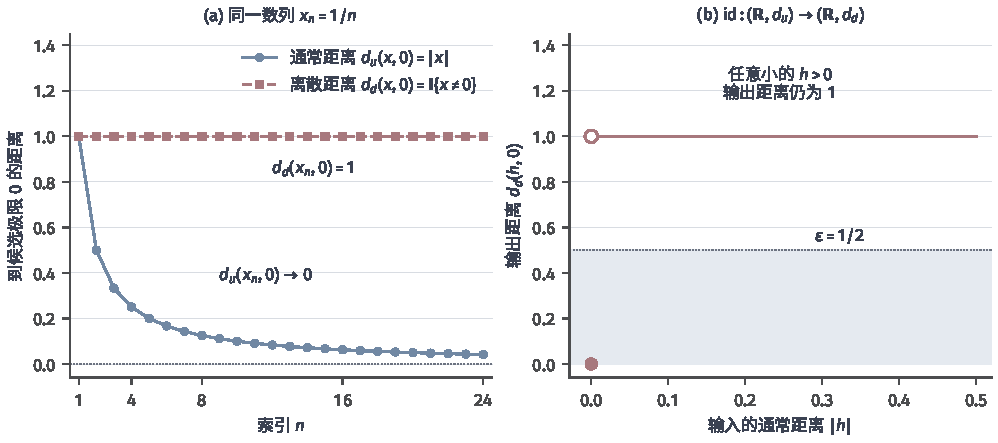
\includegraphics[width=169.0mm]{figures/01-mathematical-preliminaries-upper/01-mathematical-language-combinatorics-analysis-optimization/matplotlib/analysis-metric-convergence/figure.pdf}
 \caption{通常距离与离散距离给出不同的邻近关系，图中分别记为$d_u$和$d_d$。左图中$1/n$在通常距离下趋于$0$，在离散距离下与$0$的距离始终为$1$；右图比较恒等映射在两种距离之间的连续性。距离规则是度量空间结构的一部分。}
 \label{fig:analysis-metric-convergence}
\end{figure*}
若原集合已经给定距离，而只想取其中一部分观察，还需要说明子集怎样沿用原距离，这正是下一项的内容。

\subsubsection{子空间度量}
\label{sec:metric-subspace-metric}

将已有距离用于子集时，先确认限制规则仍然是度量，再用区间和球面说明它保留了什么、改变了什么。

\paragraph{子空间度量的定义}

只在原空间的一部分上观察点时，怎样保留原有的距离？
这里不重新规定两点的数值，而只把允许比较的点限制在子集内；
需要确认的是，缩小点的范围不会破坏度量公理。

\begin{definition}[子空间度量]
\label{def:metric-subspace}
设$(X,d)$为度量空间，$A\subseteq X$。定义
\[
  d_A=d\big|_{A\times A},\qquad d_A(x,y)=d(x,y)\quad(x,y\in A),
\]
则$(A,d_A)$也是度量空间，称为$(X,d)$的子空间，$d_A$称为\term{子空间度量}（subspace metric）。
\end{definition}

任取$A$中的两点或三点，它们同时也是$X$中的点，
所以非负性、零距离辨认、对称性和三角不等式都逐条从原空间继承；
$d_A$的值仍在$[0,\infty)$中，零距离辨认也没有因为限制点的范围而失效。
这一构造只改变允许选取的点，不改变已选两点之间的距离公式。

\paragraph{子空间度量的示例}

先取实轴中的区间$A=[0,1]$。对区间内的两点$s,t$，继承的距离仍是$|s-t|$。
端点$0,1$是否属于$A$只影响哪些点可以被选取，
不会为已经选定的两点另造距离数值；换成$(0,1)$时，内部任意两点的距离公式仍然相同。

再取欧氏空间中的球面$A=\{\bm{p}:\lVert\bm{p}\rVert_2=1\}$。
两点$\bm{p},\bm{q}$在子空间中的距离仍是环境欧氏距离$\lVert\bm{p}-\bm{q}\rVert_2$，
它等于连接两点的弦的长度，而不是沿球面行走的最短路径长度。
沿球面路径的最短长度需要用曲线长度另行定义，不能把这里继承的环境距离直接称为球面上的内蕴距离。
两个例子说明，限制到$A$以后真正改变的是球内允许出现的点：
同一个距离公式因此可能给出不同的相对邻域，下一节会把这一点写成子空间球与环境球的交集公式。

\subsection{伪距离与商度量}
\label{sec:metric-zero-distance-identification}

度量公理用零距离辨认不同对象。但有些观察规则只能看到对象的一部分特征，
天然允许不同原对象具有零距离。
本小节先放宽辨认条件，再讨论能否把不可区分的对象合并成一个新点，使合并后的类之间重新得到真正的距离。

\subsubsection{伪距离}
\label{sec:metric-pseudometric}

当观察规则忽略某些差异时，先检查剩余的距离公理是否还成立，再确定需要怎样辨认对象。

\paragraph{伪距离与不可区分对象}

从度量公理中只放宽“零距离必为同一点”这一条，其余要求全部保留，就得到伪距离。

\begin{definition}[伪距离]
\label{def:analysis-pseudometric}
设$X$为非空集合。函数$d:X\times X\to[0,\infty)$若对任意$x,y,z\in X$满足
\[
  d(x,x)=0,\qquad d(x,y)=d(y,x),\qquad d(x,z)\leq d(x,y)+d(y,z),
\]
就称为$X$上的\term{伪距离}（pseudometric，也称伪度量）。
它允许$x\neq y$时仍有$d(x,y)=0$。
\end{definition}

这里只是不再要求零距离蕴含$x=y$，并没有允许负距离，也没有破坏对称性或三角不等式。
例如在$\mathbb R^2$上令
\[
  d\bigl((x_1,x_2),(y_1,y_2)\bigr)=|x_1-y_1|.
\]
非负性、$d(x,x)=0$、对称性和三角不等式都直接来自绝对值；
但第一坐标相同、第二坐标不同的点，例如$(0,0)$与$(0,1)$，距离为零。
这个规则只记录第一坐标的差异，无法区分位于同一条竖直线上的点。

这个例子提出下一步的问题：若任务确实只区分被观察到的差异，
就应把零距离的对象归为同类，再问类与类之间的距离是否有唯一含义。
不能只凭“忽略差异”的直觉，就宣布商集上已经有了度量。

\subsubsection{零距离等价类与商度量}
\label{sec:metric-quotient-metric}

先用零距离建立等价类，再检查类之间的距离能否摆脱代表元的选择，最后把它与熟悉的例子对应起来。

\paragraph{零距离等价类}

在伪距离空间中定义
\[
  x\sim y\quad\Longleftrightarrow\quad d(x,y)=0.
\]
这一关系把被观察规则视为没有差异的对象归为同类。它确实是等价关系：
$d(x,x)=0$给出自反性，对称性给出$x\sim y\Rightarrow y\sim x$。
若$x\sim y$且$y\sim z$，则三角不等式给出
\[
  d(x,z)\leq d(x,y)+d(y,z)=0,
\]
而距离非负，故$d(x,z)=0$，即$x\sim z$，传递性成立。
记$x$所在的等价类为$[x]$，所有等价类组成商集$X/{\sim}$。

\paragraph{商度量的良定义与公理}

对两个等价类，自然想规定$\bar d([x],[y])=d(x,y)$。
但一个类里有许多代表元，必须先证明这个数值不随代表元改变。

\begin{definition}[商度量]
\label{def:metric-quotient}
在伪距离空间的商集$X/{\sim}$上定义
\begin{equation}
\label{eq:analysis-quotient-metric}
  \bar d([x],[y])=d(x,y).
\end{equation}
\end{definition}

设$x\sim u$、$y\sim v$，即$d(x,u)=d(v,y)=0$。沿新代表插入两段零距离，三角不等式给出
\[
  d(x,y)\leq d(x,u)+d(u,v)+d(v,y)=d(u,v).
\]
交换两组代表，又得到$d(u,v)\leq d(x,y)$，所以$d(x,y)=d(u,v)$，
式~\eqref{eq:analysis-quotient-metric}与代表元的选择无关，类之间的距离才有唯一含义。
非负性、对称性和三角不等式分别由原伪距离取等号或取不等式传到类上。
再由定义，
\[
  \bar d([x],[y])=0\ \Longleftrightarrow\ d(x,y)=0
  \ \Longleftrightarrow\ x\sim y\ \Longleftrightarrow\ [x]=[y],
\]
分离性被补回，所以$\bar d$是商集上的真正度量，$(X/{\sim},\bar d)$称为商度量空间。

回到只看第一坐标的例子：每个等价类
$[(a,b)]=\{(a,t):t\in\mathbb R\}$是一条竖直直线，
映射$[(a,b)]\mapsto a$把这些类一一对应到实轴，
类与类的距离就是第一坐标之差$|a-c|$。
被忽略的第二坐标并没有被恢复，而是不再作为比较对象出现。
后面的函数空间会把几乎处处相等的函数视为同一元素，
当前构造正说明了这种合并怎样消除零距离歧义；
具体的积分距离及其有限性条件，要在相应函数类上另行建立。

\section{集合的度量结构}
\label{sec:metric-set-structure}

本节固定一个度量空间$(X,d)$及其中的子集，研究集合中的点怎样分布、逼近与被覆盖。
邻域、开闭集和闭包描述一个点相对集合的位置；稠密与可分判断一个固定子集能在多大程度上代表全空间；
有界与全有界分别控制总体半径和任意精度下的覆盖数量；紧致性则进一步要求任意开覆盖都有有限子覆盖。
这些条件随后会用于判断连续映射的像与极值，以及点列能否在当前空间内取得极限。

\subsection{邻域、开闭集与闭包}
\label{sec:metric-local-set-relations}

本小节研究点与集合的邻近关系。邻域规定一个点附近的范围，开闭集把邻域判断施加于整个集合，
内部、闭包和边界描述点相对集合的位置。点到集合的距离在闭包的数值刻画中引入；
距离下确界是否由某一点达到，则留到后面紧致集上的映射应用中研究。

\subsubsection{邻域与相对邻域}
\label{sec:metric-neighborhoods}

先固定当前度量空间中的球与邻域，再缩小到子空间，说明同一个距离公式为何会产生不同的相对邻域。

\paragraph{开球与邻域}

如何用距离阈值精确表达“在一个点附近”？
给定中心点和正的半径，可以把所有足够接近中心的点收集成一个集合。

\begin{definition}[开球与邻域]
\label{def:metric-open-ball}
设$(X,d)$为度量空间，$x\in X$，$r>0$。集合
\[
  B(x,r)=\{y\in X:d(x,y)<r\}
\]
称为以$x$为中心、以$r$为半径的开球。
若集合$V\subseteq X$包含某个开球$B(x,r)$，即存在$r>0$使$B(x,r)\subseteq V$，就称$V$为$x$的一个邻域。
\end{definition}

开球的定义里要注意两点：不等式是严格的$d(x,y)<r$，半径$r$必须为正。
球的形状取决于度量：实轴上的球是开区间，欧氏平面上的球是圆盘，
离散空间中半径小于$1$的球只含中心一个点。
邻域只需包含某个开球，本身不必是开集，也不能因为含有$x$就自动成为$x$的邻域；
例如实轴上的闭区间$[0,1]$是其内点$1/2$的邻域，却不是端点$0$的邻域。
图~\ref{fig:analysis-ball-neighborhood}已在平面欧氏距离下把这两个对象分开画出。

开球中的每一点都带有一个完全落在该球内的小球。若$y\in B(x,r)$，令
\[
  \rho=r-d(x,y)>0,
\]
则对任意$z\in B(y,\rho)$，三角不等式给出
$d(x,z)\leq d(x,y)+d(y,z)<d(x,y)+\rho=r$，所以
\begin{equation}
\label{eq:metric-ball-is-open}
  B(y,\rho)\subseteq B(x,r).
\end{equation}
这一性质为下一项的开放性提供了局部理由，也提醒所有球都只在当前空间$X$中取点。

\paragraph{相对邻域}

同一个点在大空间和子空间中，为什么会有不同的邻域判断？
沿用\ref{sec:metric-subspace-metric}节的子空间度量可以直接比较两种球。

设$A\subseteq X$配备子空间度量$d_A$。为区分所在空间，把$A$中的球记为$B_A(x,r)$，把$X$中的球记为$B_X(x,r)$。由定义，
\begin{equation}
\label{eq:metric-relative-ball}
  B_A(x,r)=A\cap B_X(x,r)\qquad(x\in A,\ r>0),
\end{equation}
因为两边都恰好表示“属于$A$且与$x$的环境距离小于$r$”的点。距离数值没有改变，改变的是可取点的范围。

取$A=[0,1]\subseteq\mathbb R$和端点$0$。在子空间$A$中，$0$的一个小球是
\[
  B_A(0,r)=[0,r)\cap A,
\]
它包含$0$右侧一段属于$A$的点；但在实轴$\mathbb R$中，任何$B_{\mathbb R}(0,r)=(-r,r)$都含有负数，
因而$[0,r)\cap A$不可能包含任何围绕$0$的实轴球。
于是同一个集合是否为$0$的邻域，要附属于所在空间来回答。
对$x\in A$，$V\subseteq A$是$x$在$A$中的邻域，当且仅当它包含某个相对球$B_A(x,r)$。
这也预示开放与封闭同样要相对当前空间判断，不能把端点处的几何直觉直接当成一般定义。

\subsubsection{开集与闭集}
\label{sec:metric-open-and-closed}

把“点附近有一个球”的条件用于整个集合，就得到开集；对补集作同样检验，则得到闭集。

\paragraph{开闭集的邻域判据}

\begin{definition}[开集与闭集]
\label{def:metric-open-closed}
设$(X,d)$为度量空间，$U\subseteq X$。若对每个$x\in U$都存在$r>0$使$B(x,r)\subseteq U$，
就称$U$为开集。若补集$X\setminus U$是开集，就称$U$为闭集。
\end{definition}

定义中的半径允许随点改变：不同位置可以使用大小不同的球，只要求每个点各自拥有一个。
用实轴的开区间可以直接检验：每个内点都能取一个完全落在区间内的小球。
在离散空间中，任意子集都是开集，因为半径小于$1$的球只含中心，必然包含在该子集中；
其补集同样任意，所以离散空间的任意子集同时也是闭集。

把闭集的定义改写一次，更便于使用：$F$为闭集，当且仅当每个$x\notin F$都有一个球完全避开$F$。
这是因为$X\setminus F$为开集，恰好表示每个外点都被某个球包在补集内部。
这里先用补集关系解释闭性；闭集的序列判据要到点列语言建立后再证明，不用尚未建立的等价表述代替定义。

空集和全空间$X$既开又闭：空集没有需要检验的点，而每个$x\in X$都有包含于$X$的球，两者的补集也满足同样条件。
但不能由此认为所有集合非开即闭。在$\mathbb R$中，$[0,1)$不是开集，因为$0$处没有完全落在集合内的小球；它也不是闭集，因为外点$1$无法用一个球避开$[0,1)$。
图~\ref{fig:analysis-open-closed-relative}用实轴区间和子空间中的端点检验了这种对环境的依赖。

由式~\eqref{eq:metric-ball-is-open}可知每个开球都是开集：球内任一点都有完全包含于该球的小球。
进一步，任意多个开集的并仍是开集，因为并集中每个点都已属于其中某个开集，可以沿用它的球；
有限多个开集的交仍是开集，因为可取各点在这些开集中所得半径的最小值。
“有限”不能改成“任意”，例如
\[
  \bigcap_{n\geq1}\Bigl(-\frac1n,\frac1n\Bigr)=\{0\},
\]
每个区间都是开集，其交集$\{0\}$却不是开集。

\subsubsection{内部、闭包与边界}
\label{sec:metric-interior-closure-boundary}

下面先用邻域描述点相对集合的位置，再把这些位置条件改写成数值距离判据，最后在区间和子空间中核对。

\paragraph{内部、闭包与边界的邻域判据}

设$A\subseteq X$。若存在$r>0$使$B(x,r)\subseteq A$，就称$x$为$A$的\term{内点}（interior point）；
全部内点组成$A$的内部，记作$A^\circ$。
按定义有$A^\circ\subseteq A$。若$B(x,r)\subseteq A$，则球内每一点$y$又可由式~\eqref{eq:metric-ball-is-open}取一个留在$B(x,r)$中的小球，因而$y$也是内点；
这说明整个$B(x,r)$都包含在$A^\circ$中，内部$A^\circ$是开集。
于是$A$为开集时每个$x\in A$都是内点，即$A^\circ=A$；反之，若$A=A^\circ$，由内部为开集得到$A$为开集。

闭包描述的是另一种位置：若每个正半径球都与$A$相交，就称$x$为$A$的闭包点，全部闭包点组成\term{闭包}（closure）$\overline A$，即
\[
  \overline A=\{x\in X:\forall r>0,\ B(x,r)\cap A\neq\varnothing\}.
\]
显然$A\subseteq\overline A$。与内点要求“存在一个球包含于集合”相比，闭包要求“每一个球都接触集合”，所以闭包点不必已经属于$A$。
闭包本身是闭集。事实上，若$x\notin\overline A$，则存在$r>0$使$B(x,r)\cap A=\varnothing$。
对任意$y\in B(x,r/2)$，$B(y,r/2)\subseteq B(x,r)$也避开$A$，故$y\notin\overline A$。
这说明补集$X\setminus\overline A$中每点都有一个球留在补集中，所以$X\setminus\overline A$为开集。

由此可以建立$A$为闭集与$A=\overline A$的等价关系。若$A$为闭集而$x\notin A$，外点$x$拥有避开$A$的球，故$x\notin\overline A$，得到$\overline A\subseteq A$；连同$A\subseteq\overline A$，有$A=\overline A$。
反过来，若$A=\overline A$，而闭包已经证明为闭集，所以$A$为闭集。
这个等价关系会在后面的距离判据与点列判据中反复使用。

边界点要求每个球同时碰到$A$和它的补集$X\setminus A$，全部边界点记作$\partial A$。按定义，
\[
  \partial A=\overline A\cap\overline{X\setminus A}.
\]
又因为$x\notin A^\circ$恰好表示每个球都碰到补集，所以$\overline{X\setminus A}=X\setminus A^\circ$，从而
\begin{equation}
\label{eq:metric-boundary-difference}
  \partial A=\overline A\setminus A^\circ.
\end{equation}
内部、闭包和边界因此都能用同一族球刻画，区别只在球是包含于集合、接触集合，还是同时接触两侧。

\paragraph{点到集合的距离}

“每个球都碰到$A$”是一种球条件，还可以换成数值判据。
对非空集合$A$定义点$x$到$A$的距离
\begin{equation}
\label{eq:metric-distance-to-set}
  d(x,A)=\inf_{a\in A}d(x,a).
\end{equation}
由于候选距离非负，且任取一个$a_0\in A$便有$d(x,A)\leq d(x,a_0)<\infty$，
所以这个下确界是有限的非负数。它具有两条与下确界相符的性质：
每个候选距离都不小于$d(x,A)$；对任意$\varepsilon>0$，又都能选到$a\in A$使
\begin{equation}
\label{eq:metric-infimum-approx}
  d(x,a)<d(x,A)+\varepsilon.
\end{equation}
这种近似性质并不要求某个点恰好达到下确界。为统一叙述，约定$d(x,\varnothing)=+\infty$。

点到集合的距离随点的移动满足 Lipschitz 型估计。对非空$A$和任意$x,y$，
\[
  d(x,a)\leq d(x,y)+d(y,a)\qquad(a\in A).
\]
对右侧候选取下确界，得到$d(x,A)\leq d(x,y)+d(y,A)$；交换$x,y$再得反向不等式，故
\begin{equation}
\label{eq:metric-set-distance-lipschitz}
  \bigl|d(x,A)-d(y,A)\bigr|\leq d(x,y).
\end{equation}
这个估计说明距离函数随点连续变化，后面会用于连续性和极值问题。

更重要的是，距离为零恰好刻画闭包。对非空$A$，
\begin{equation}
\label{eq:metric-zero-distance-closure}
  x\in\overline A\quad\Longleftrightarrow\quad d(x,A)=0.
\end{equation}
若$d(x,A)=0$，则由式~\eqref{eq:metric-infimum-approx}，对每个$r>0$都能选到$a\in A$使$d(x,a)<r$，即$B(x,r)\cap A\neq\varnothing$；
反过来，若每个球都与$A$相交，则$d(x,A)<r$对所有$r>0$成立，而距离非负，故$d(x,A)=0$。
当$A$为闭集时，再用$A=\overline A$得到
\[
  d(x,A)=0\quad\Longleftrightarrow\quad x\in A.
\]
这些数值结论都是由球定义推出的，并没有另换闭包的含义。

\paragraph{区间的内部、闭包与边界}

在实轴上计算$(0,1)$和$[0,1]$，可以看到内部与闭包分别回答什么问题。两者的内部都是$(0,1)$，闭包都是$[0,1]$，边界都是$\{0,1\}$。
对开区间的端点，任意小球都碰到区间和补集，所以端点属于边界和闭包，却不属于内部或原集合；固定一个内部点，则能取足够小的球完全留在区间内。

换到子空间时，所有球都要改用相对球，结论也随之改变。$[0,1]$在它自身中的内部是整个$[0,1]$，因为端点处的相对球不必包含负数；这与它在实轴中的内部$(0,1)$不同。
再回看开区间的端点：$d(0,(0,1))=0$说明可以任意逼近，却不表示下确界由区间内某点达到。最近点要求式~\eqref{eq:metric-distance-to-set}的下确界由$A$中的点真正达到，这是在距离数值之外新增的存在性条件，将在紧致集的极值应用中研究。

\subsection{稠密子集与可分空间}
\label{sec:metric-countable-approximation}

固定一个代表子集，先研究它能否逼近空间中的所有点，再增加代表数量可数的要求。

\paragraph{稠密子集的判据与构造}

\begin{definition}[稠密子集]
\label{def:metric-dense}
设$D\subseteq X$。若$\overline D=X$，就称$D$在$X$中\term{稠密}（dense）。
\end{definition}

由闭包的球判据，稠密性等价于：对每个$x\in X$和每个$\varepsilon>0$，都能选到$a\in D$使$d(x,a)<\varepsilon$。
度量空间和被逼近的整个$X$保持固定，所选代表$a$可以随位置$x$与精度$\varepsilon$改变，不要求用同一个点应付所有情形。

有理数集$\mathbb Q$在实轴上稠密。给定$x\in\mathbb R$和$\varepsilon>0$，先取正整数$m$使$1/m<\varepsilon$，再选整数$k$满足
\[
  \frac{k}{m}\leq x<\frac{k+1}{m}.
\]
于是$0\leq x-k/m<1/m<\varepsilon$，所以有理点$k/m$落在$B(x,\varepsilon)$中。
这个构造是实际选出代表，而不是只凭$\mathbb Q$含有无限多个点下判断；一般空间中也要在每个球里找到代表，集合无限本身并不推出稠密。

稠密并不意味着集合含有一个非空开球。考虑任意开区间$(\alpha,\beta)$，把其中点作为$x$、取小于半长的精度，上一构造先给出区间内的有理点$q$。
再取充分大的正整数$n$使$\sqrt2/n<\beta-q$，则$q+\sqrt2/n$仍是区间中的无理数。
因此每个实轴小球既碰到$\mathbb Q$，也碰到它的补集，由内部、闭包和边界的判据得到
\[
  \mathbb Q^\circ=\varnothing,\qquad \overline{\mathbb Q}=\mathbb R,\qquad \partial\mathbb Q=\mathbb R.
\]
点可以任意接近$D$，与$D$是否包含一小片完整邻域，是两种不同的性质。

\paragraph{可分空间与可数代表}

在稠密性上再增加代表集可数的要求，就得到可分性。

\begin{definition}[可分空间]
\label{def:metric-separable}
若度量空间$X$存在一个可数的稠密子集$D$，就称$X$\term{可分}（separable）。
\end{definition}

这里要求同一套可数代表同时服务所有位置与精度，不能每次另换一套集合；
但对每个具体精度，仍可以使用$D$中不同的点，定义并不要求只靠有限多个代表。
若$X$本身可数，取$D=X$便说明$X$可分；但反方向不成立，因为不可数的$\mathbb R$具有可数稠密集$\mathbb Q$。
这里区分的是全部点的数量与代表点的数量，而不是两种不同的稠密定义。

不可数离散空间给出反例。在离散度量下，半径小于$1$的球都只含中心一个点；
稠密集必须碰到每个这样的单点球，因而只能等于整个不可数空间。所以不可数离散空间不可分。
与通常度量下的实轴对照可见，可分性取决于当前距离决定的邻近关系，而不只取决于底层集合的大小。

可分性允许一套可数代表应对所有精度。若换一种更强的条件，使每个精度都只需有限多个代表，
就能把各精度的有限代表取可数并，构造出这样一套可数稠密集。下面据此研究有限覆盖的要求。
还要注意，集合能被代表点逼近，并没有说明任意点列都能取得空间内的极限，后一个保证属于\ref{sec:metric-completeness}节。

\subsection{有界集与有限覆盖}
\label{sec:metric-covering-budgets}

本节固定集合及其子空间度量，先问能否用一个有限半径的球容纳整个集合，
再问每个指定精度下能否只用有限多个小球覆盖。
前者控制总体半径，后者控制任意小尺度下的代表数量；
把各精度的有限代表汇合，还能建立全有界与可分性之间的联系。

\subsubsection{有界集}
\label{sec:metric-boundedness}

从“一个有限半径的球能否容纳全体点”进入有界性，再用直径刻画同一要求。

\paragraph{有界性与直径}

\begin{definition}[有界集与直径]
\label{def:metric-bounded}
设$(X,d)$为度量空间，$A\subseteq X$。若存在中心$x_0\in X$和有限半径$R>0$使$A\subseteq B(x_0,R)$，就称$A$为\term{有界集}（bounded set）；空集按约定有界。
对非空$A$，定义直径
\[
  \operatorname{diam}A=\sup\{d(x,y):x,y\in A\},
\]
允许上确界为$+\infty$，$\operatorname{diam}A$读作集合的\term{直径}（diameter）；并约定$\operatorname{diam}\varnothing=0$。
\end{definition}

定义中中心是否取在$A$内不影响判断。若$A\subseteq B(x_0,R)$，任取固定点$a_0\in A$，由三角不等式
\[
  d(x,a_0)\leq d(x,x_0)+d(x_0,a_0)<2R\qquad(x\in A),
\]
换到以$a_0$为中心只需增大半径。

有界性与直径有限等价。若$A\subseteq B(x_0,R)$，则任意两点满足$d(x,y)<2R$，所以$\operatorname{diam}A\leq2R$。
反过来，若直径$D=\operatorname{diam}A<\infty$，固定$a_0\in A$，则$d(x,a_0)\leq D$对所有$x\in A$成立，
取任意半径$D+\varepsilon$（$\varepsilon>0$）便得到容纳$A$的开球。
对空集的两项约定也彼此相容。

实轴上的有限区间有界，全实轴无界。更有启发性的反例是无限离散空间：
任意不同点的距离都是$1$，所以整个空间包含在任一半径大于$1$的球中，仍然有界。
这说明有界只控制总体半径，并未保证在更小精度下只需有限多个代表点。

\subsubsection{全有界与有限$\varepsilon$网}
\label{sec:metric-total-boundedness}

先建立每个精度下的有限网要求，再说明它比有界更强，最后把一系列有限网汇成可数稠密集。

\paragraph{全有界与有限网}

\begin{definition}[全有界与有限$\varepsilon$网]
\label{def:metric-totally-bounded}
设$A$配备子空间度量。若对每个$\varepsilon>0$，都存在有限个中心$a_1,\ldots,a_N\in A$，使
\[
  A\subseteq\bigcup_{i=1}^{N}B_A(a_i,\varepsilon),
\]
就称$A$\term{全有界}（totally bounded），并称$\{a_1,\ldots,a_N\}$为$A$的一个\term{有限网}（finite net）。
\end{definition}

精度改变时可以重新选择有限网，定义并不要求一套固定的有限网同时控制所有精度；
但对每一个固定精度，代表的数量必须有限。

全有界推出有界。固定一个精度，例如$\varepsilon=1$，并取有限网$a_1,\ldots,a_N$。
令$M=\max_i d(a_1,a_i)$。每个$x\in A$都属于某个$B_A(a_i,1)$，于是
\[
  d(x,a_1)\leq d(x,a_i)+d(a_i,a_1)<1+M,
\]
所以整个$A$包含在以$a_1$为中心的有限半径球内。空集可用空覆盖处理，不必强选中心。

有界却不一定全有界。无限离散空间虽有界，但取$\varepsilon<1$时每个球只含中心一个点，
覆盖整个空间需要无限多个中心。
再看实轴上的有界区间：把区间分成有限个长度小于$\varepsilon$的小段，
从每个与区间相交的小段中选一个区间内的点，则同一段中任意两点距离小于$\varepsilon$，
这些选点构成有限$\varepsilon$网。论证对未封闭区间同样成立，网点不必选在被排除的端点上。

\paragraph{由有限网构造可数稠密集}

每个精度的有限覆盖，怎样汇成一套能逼近所有点的可数代表？

设$A$全有界。对每个$n\geq1$选取一个有限$2^{-n}$网$F_n$，并令
\[
  D=\bigcup_{n\geq1}F_n.
\]
每个$F_n$都是有限集，可数个有限集的并仍可数，所以$D$是可数集；
合并后得到的是一套固定代表集，但它一般不再有限。

给定$x\in A$和$\varepsilon>0$，先选$n$使$2^{-n}<\varepsilon$，再由$F_n$的覆盖性选$a\in F_n$满足
$d(x,a)<2^{-n}<\varepsilon$。由于$F_n\subseteq D$，每个$B(x,\varepsilon)$都碰到$D$，所以$D$在$A$中稠密。
因此全有界空间可分。

反方向不成立：通常度量下的$\mathbb R$可分，却不是有界的，而全有界已经推出有界，故$\mathbb R$不全有界。
此后若另一个条件保证每个精度都存在有限球覆盖，就可以直接使用上述构造得到可数稠密集。

\subsection{紧致集与有限子覆盖}
\label{sec:metric-compact-control}

把“每个精度重选有限球”的要求，与“从任意既定开覆盖中选有限成员”的要求比较，就得到紧致性。

\paragraph{紧致性的开覆盖定义}

\begin{definition}[开覆盖、有限子覆盖与紧致性]
\label{def:metric-compactness}
设$K$为度量空间$X$的子集，并把$K$自身作为配备继承距离的度量空间。
若一族在$K$中相对开的集合$\{U_\alpha\}_{\alpha\in I}$满足
\[
  K\subseteq\bigcup_{\alpha\in I}U_\alpha,
\]
就称这族集合为$K$的相对开覆盖；若其中有限多个成员的并仍包含$K$，就称它们构成有限子覆盖。
若$K$的每个开覆盖都有有限子覆盖，就称$K$紧致。
\end{definition}

有限子覆盖只能从原有覆盖成员中选取，不能另换一组集合；开覆盖本身可以含有无限多个成员。
空集由空子覆盖满足条件，按约定紧致。

\paragraph{紧致集的有限网与闭性}

固定$\varepsilon>0$，全部相对球$\{B_K(a,\varepsilon):a\in K\}$构成$K$的一个开覆盖。
若$K$紧致，就能从中选出有限个球覆盖$K$，它们的中心恰好给出一个有限$\varepsilon$网，所以紧致推出全有界。
再回用前面的两项构造：一次固定精度的覆盖控制总体半径，故紧集有界；
各精度有限网的可数并提供可数稠密集，故紧集可分。

紧集在环境空间中还是闭集。设$K$非空紧致，$x\in X\setminus K$。对每个$a\in K$令
\[
  r_a=\frac{d(x,a)}{3}>0,
\]
则相对集合$K\cap B_X(a,r_a)$覆盖$K$。由紧致性，可选出有限个中心$a_1,\ldots,a_N$，使这些相对球覆盖$K$。令
\[
  r=\min_{1\leq i\leq N}r_{a_i}>0.
\]
对$y\in B_X(x,r)$和每个$i$，三角不等式给出
\[
  d(y,a_i)\geq d(x,a_i)-d(x,y)>d(x,a_i)-r\geq d(x,a_i)-r_{a_i}=2r_{a_i}>r_{a_i},
\]
所以$B_X(x,r)$避开每个$B_X(a_i,r_{a_i})$，也避开被它们覆盖的$K$。
每个外点都有这样一个球，说明$X\setminus K$为开集，故$K$为闭集；
$K$为空时其补集为$X$，同样为闭集。

\paragraph{有界与全有界不保证紧致}

在一般度量空间中，闭且有界不足以推出紧致。
无限离散空间的整个空间既闭又有界，但由全部单点开集构成的开覆盖没有有限子覆盖，
因为每个单点开集只能覆盖一个点。这里有限半径不能限制小尺度覆盖所需的数量，与全有界失败的原因相同。

全有界也仍不够。通常度量下$K=(0,1)$已由有限个小段覆盖证明为全有界。考虑
\[
  U_n=\Bigl(\frac1n,1\Bigr),\qquad n\geq2.
\]
每个$U_n$在$K$中相对开；对任意$x\in K$，选$n>1/x$便有$x\in U_n$，所以$\{U_n\}_{n\geq2}$覆盖$K$。
但任取有限多个成员后，设$N$是其中最大的指标，它们的并仍只是$U_N$，遗漏了$1/(2N)\in K$。
故$K$不紧致，由全有界推出的可分性也不能代替紧致。

这个覆盖失败与点列缺少怎样的极限点有关。
全有界还要增加什么极限保证才能得到紧致，欧氏空间中闭且有界为何足够，
都要在\ref{sec:metric-compactness-tests}节结合点列与完备性说明。
图~\ref{fig:analysis-process-finite-open-cover}已经把闭区间的有限覆盖与这里的开区间失败覆盖画在一起，可对照观察有限子覆盖遗漏的位置。

\section{映射的连续性与距离控制}
\label{sec:metric-map-error-transfer}

固定映射以后，输入误差怎样限制输出误差，输出又能保留多少输入差异？
本节从一个基点附近的函数极限与连续性出发，比较全域共用半径和比例上界两种控制；
再加入比例下界，研究像上逆映射的误差。
紧致定义域还会使连续像保持紧致、实值输出达到极值，并把各点的连续控制合成为统一控制。

\subsection{函数极限与连续性}
\label{sec:metric-map-limits}

先固定两个度量空间及它们之间的映射，研究输入接近一个基点时输出能否接近一个确定目标，
以及这个目标与基点处函数值之间是什么关系。

\paragraph{函数极限与唯一性}

固定度量空间$(X,d_X)$、$(Y,d_Y)$和映射$f:D\subseteq X\to Y$。
为使输入确实能够穿过其他点接近$a\in X$，要求每个$\delta>0$都存在$x\in D$满足$0<d_X(x,a)<\delta$；
这正是第~\ref{sec:analysis-function-limits}节已经引入的聚点条件，这里把$a$称为$D$的聚点。

\begin{definition}[函数极限]
\label{def:metric-function-limit}
设$a$是$D$的聚点。若对候选$L\in Y$，每个$\varepsilon>0$都存在$\delta>0$，使
\[
  x\in D,\quad 0<d_X(x,a)<\delta
  \quad\Longrightarrow\quad d_Y(f(x),L)<\varepsilon,
\]
就称$x\to a$时$f(x)$趋于$L$，记作$\lim_{x\to a}f(x)=L$。
\end{definition}

这里$a$可以不属于$D$，条件也不使用$f(a)$；穿孔限制$0<d_X(x,a)$把基点本身排除在外。
这个输出目标若存在就是唯一的。若不同的$L_1,L_2$都满足极限条件，令
$\eta=d_Y(L_1,L_2)/3>0$，分别按$\eta$取得输入半径，再取两者中较小的一个$\delta$。
聚点条件保证穿孔小球$B_D(a,\delta)\setminus\{a\}$中仍有合法输入$x$。于是
\[
  d_Y(L_1,L_2)
  \leq d_Y(L_1,f(x))+d_Y(f(x),L_2)<2\eta,
\]
而$d_Y(L_1,L_2)=3\eta$，矛盾。聚点条件负责排除“没有输入可检验”的空条件；
它并不保证极限一定存在，只保证一旦存在就不会有两个不同目标。

\paragraph{连续与函数值}

当$a\in D$时，可以把候选目标换成基点处的函数值。

\begin{definition}[连续]
\label{def:metric-continuity-at-point}
设$f:D\subseteq X\to Y$，$a\in D$。若对每个$\varepsilon>0$都存在$\delta>0$，使
\[
  x\in D,\quad d_X(x,a)<\delta
  \quad\Longrightarrow\quad d_Y(f(x),f(a))<\varepsilon,
\]
就称$f$在$a$连续。若$f$在$D$的每一点都连续，就称$f$连续。
\end{definition}

在$a$也是$D$的聚点时，连续性与函数极限的关系很直接。
连续条件限制到穿孔输入便得到极限等于$f(a)$；反过来，若$\lim_{x\to a}f(x)=f(a)$，
同一个半径已经控制所有穿孔输入，而$x=a$时输出误差为零，故$f$在$a$连续。
因此在聚点处，
\[
  f\text{ 在 }a\text{ 连续}\quad\Longleftrightarrow\quad\lim_{x\to a}f(x)=f(a).
\]
若穿孔极限存在却不等于$f(a)$，极限的唯一性也排除了连续的可能。

若$a$是$D$中的孤立点，即存在$r>0$使$B_X(a,r)\cap D=\{a\}$，
则在这个半径内只有基点自身需要检验，$f$自动在$a$连续。
但相应的穿孔小球中没有输入，无论指定哪个$L\in Y$，定义~\ref{def:metric-function-limit}的阈值式都会空泛成立；
所以孤立点处不按聚点定义使用函数极限，也不能由这种空条件断言唯一的输出目标。
连续性的定义仍然适用于这样的定义域点。

\subsection{一致连续与Lipschitz条件}
\label{sec:metric-uniform-continuity}

在一点连续时，控制输入误差的半径可以随基点变化。
下面固定$f:D\subseteq X\to Y$及两端度量，比较何时能够共用一个半径，
以及何时能够用输入距离的固定比例控制输出距离。

\paragraph{逐点连续与一致连续}

逐点连续允许对每个基点$a\in D$和每个$\varepsilon>0$分别选择$\delta(a,\varepsilon)>0$。
一致连续则把半径提到基点之前：

\begin{definition}[一致连续]
\label{def:metric-uniformly-continuous}
设$f:D\subseteq X\to Y$。若对每个$\varepsilon>0$都存在$\delta>0$，使任意$x,y\in D$满足
\[
  d_X(x,y)<\delta\quad\Longrightarrow\quad d_Y(f(x),f(y))<\varepsilon,
\]
就称$f$在$D$上一致连续。
\end{definition}

后者要求同一个输入容差同时服务全域的所有输入对，因此一致连续推出$f$在每个基点处连续；
反方向一般不成立。用通常绝对值距离下的$f(x)=x^2$检验这一区别。
在基点$a$附近，$|x-a|<1$时
\[
  |x^2-a^2|=|x+a|\,|x-a|\leq(2|a|+1)|x-a|,
\]
取$\delta=\min\{1,\varepsilon/(2|a|+1)\}$便得到逐点连续，但这个半径随$a$增大。
为说明全实轴上不一致连续，固定输出容差$\varepsilon_0=1$。任给$\delta>0$，取
\[
  x>\max\!\left\{1,\frac1\delta\right\},\qquad y=x+\frac1x.
\]
则$|x-y|=1/x<\delta$，而
\[
  |x^2-y^2|=(y-x)(x+y)=\frac1x\Bigl(2x+\frac1x\Bigr)=2+\frac1{x^2}>1,
\]
所以每个候选统一半径都会遇到失败的输入对。

\paragraph{Lipschitz控制与连续性条件的关系}

一种取得统一半径的办法，是要求输出距离始终不超过输入距离的固定倍数。

\begin{definition}[全局Lipschitz条件]
\label{def:metric-lipschitz}
设$f:D\subseteq X\to Y$。若存在有限常数$L\geq0$，使所有$x,y\in D$满足
\begin{equation}
\label{eq:metric-lipschitz}
  d_Y(f(x),f(y))\leq L\,d_X(x,y),
\end{equation}
就称$f$满足全局Lipschitz条件，$L$称为一个Lipschitz常数。
\end{definition}

当$L>0$时，给定$\varepsilon>0$取$\delta=\varepsilon/L$，便得到一致连续；
当$L=0$时，任意两输入的输出距离为零，输出相同，也一致连续。
因此比例上界是比共用半径更具体的控制方式。

若全域共用常数过强，还可以只要求每个基点附近存在自己的比例常数：
存在$r_a>0$与有限$L_a\geq0$，使所有$x,y\in D\cap B_X(a,r_a)$满足
$d_Y(f(x),f(y))\leq L_a d_X(x,y)$。这称为局部Lipschitz条件。
令其中一个输入为$a$，便得到$f$在$a$连续；但不同基点的常数未必能合成一个全域常数。

仍以平方函数为例。固定$a$和$r>0$，邻域内$|x+y|\leq2(|a|+r)$，所以
\[
  |x^2-y^2|\leq 2(|a|+r)|x-y|,
\]
它在实轴上局部Lipschitz；前面的全实轴反例又说明它并不一致连续。
若把同一函数限制到$[0,1]$，则$|x+y|\leq2$给出全局Lipschitz常数$2$及一致连续，
说明定义域的范围本身也是条件的一部分。

再用$[0,1]$上的$f(x)=\sqrt x$检验一致连续能否反推Lipschitz。对$x>y$，
\[
  |\sqrt x-\sqrt y|=\frac{x-y}{\sqrt x+\sqrt y}.
\]
由$\sqrt x+\sqrt y\geq\sqrt{x-y}$，交换$x,y$并处理相等情形后可得
\[
  |\sqrt x-\sqrt y|\leq\sqrt{|x-y|},
\]
取$\delta=\varepsilon^2$便能统一控制输出，所以根号函数一致连续。
另一方面，$0$的任意相对邻域都含充分小的正$x$，而
\[
  \frac{|\sqrt x-\sqrt0|}{|x-0|}=\frac1{\sqrt x}
\]
在每个这样的邻域中无界，故它在$0$处不局部Lipschitz，也不存在全域Lipschitz常数。

综合起来，实际蕴含关系是
\[
  \text{全局Lipschitz}\Longrightarrow\text{一致连续}\Longrightarrow\text{连续},
\]
全局Lipschitz也推出局部Lipschitz，局部Lipschitz推出逐点连续；
但一致连续与局部Lipschitz之间没有一般蕴含关系：
$[0,1]$上的根号函数排除了“一致连续推出局部Lipschitz”，
全实轴上的平方函数排除了“局部Lipschitz推出一致连续”。
这些判断都针对已经固定的函数、定义域和两端度量，不能在改变范围后沿用同一结论。
第~\ref{chap:univariate-calculus}章在一元实函数情形还会引入绝对连续，
它控制许多小区间上的总增量，与这里的两个条件不是同一种要求。

\subsection{等距与双Lipschitz映射}
\label{sec:metric-isometry-bilipschitz}

式~\eqref{eq:metric-lipschitz}的比例上界仍允许不同输入落到同一输出：
常值映射满足Lipschitz上界，却无法从输出辨认输入。
若还要求输出距离至少保留输入距离的一个固定正比例，就需要加入下界，
它同时给出像上逆映射的Lipschitz误差控制。

\begin{definition}[等距映射与双Lipschitz映射]
\label{def:metric-isometry-bilipschitz}
设$f:D\subseteq X\to Y$。若
\[
  d_Y(f(x),f(y))=d_X(x,y)\qquad(x,y\in D),
\]
就称$f$为\term{等距映射}（isometry）。若存在常数$0<c\leq C<\infty$，使所有$x,y\in D$满足
\begin{equation}
\label{eq:metric-bilipschitz}
  c\,d_X(x,y)\leq d_Y(f(x),f(y))\leq C\,d_X(x,y),
\end{equation}
就称$f$为\term{双Lipschitz映射}（bi-Lipschitz mapping）。
\end{definition}

若$f(x)=f(y)$，下界给出$c\,d_X(x,y)\leq0$，而$c>0$，故$d_X(x,y)=0$；
再用度量的分离性得到$x=y$，所以双Lipschitz映射（包括等距映射）是单射。
于是可以在像$f(D)$上定义逆映射$f^{-1}$。对像内的$u=f(x)$、$v=f(y)$，重排下界得到
\begin{equation}
\label{eq:metric-inverse-lipschitz}
  d_X\bigl(f^{-1}(u),f^{-1}(v)\bigr)\leq\frac1c\,d_Y(u,v).
\end{equation}
这说明输出误差如何限制可恢复输入的误差；等距映射正是两侧常数都为$1$的特例。
逆映射的定义域始终是配备子空间度量的$f(D)$；在没有满射到整个$Y$的条件时，不能把它替换成整个$Y$。

实轴上的正比例缩放$f(t)=st$（$s>0$）满足式~\eqref{eq:metric-bilipschitz}，两侧常数都是$s$。
包含映射$j:(0,1)\to\mathbb R$，$j(t)=t$，则是等距映射，但它的像只是$(0,1)$，没有覆盖整个陪域。
两个例子分别检查距离比例与映射范围：不能仅凭等距，就把定义域的性质推广到整个陪域。
点列的收敛与柯西条件建立以后，还会把同一两侧距离界用于点列，
检验误差能否正反传递以及极限是否留在像中。

\subsection{紧致定义域上的连续映射}
\label{sec:metric-compactness-consequences}

固定紧致集合$K$及连续映射$f:K\to Y$。
本节先判断连续像是否紧致、实值输出能否达到极值，再把各点的连续半径合成一个统一半径。
极值路线利用像的闭性和实数的确界，最近点则把这一路线用于距离函数最小化；
一致连续路线利用有限球覆盖合并各点的误差控制。

\subsubsection{连续像与极值}
\label{sec:metric-continuous-images-extrema}

先证明连续像保持紧致，再讨论实值函数的最大值、最小值以及最近点的存在与非唯一。

\paragraph{连续像的紧致性}

设$K$紧致、$f:K\to Y$连续。要证明像$f(K)$紧致，先看$f$怎样把像中的相对开集拉回定义域。
设$U$是$f(K)$中的相对开集，且$f(x)\in U$。存在$r>0$使
\[
  B_Y(f(x),r)\cap f(K)\subseteq U.
\]
由$f$在$x$连续，可取$K$中的输入球，使其中点的输出都落入$B_Y(f(x),r)$；这些输出本就属于$f(K)$，因此仍属于$U$。这说明原像$f^{-1}(U)$在$K$中相对开。

现在任取$f(K)$的一个相对开覆盖$\{U_\alpha\}$。由上一步，$\{f^{-1}(U_\alpha)\}$是$K$的开覆盖；
$K$紧致，故有有限子覆盖$f^{-1}(U_{\alpha_1}),\ldots,f^{-1}(U_{\alpha_N})$。
对应的$U_{\alpha_1},\ldots,U_{\alpha_N}$覆盖$f(K)$，所以$f(K)$紧致。
证明不要求$f$单射，也不要求像覆盖整个$Y$。

\paragraph{实值函数的极值}

\begin{theorem}[紧集上实值连续函数的极值]
\label{thm:metric-extreme-value}
设$K$非空紧致，$f:K\to\mathbb R$连续，并使用实轴通常距离。则$f(K)$是$\mathbb R$中的非空紧集，
$f$在$K$上达到最大值和最小值。
\end{theorem}

\begin{proof}
由连续像的紧致性，$f(K)$紧致，而紧集在度量空间中闭且有界，所以$f(K)$是有界闭集。
令$M=\sup f(K)$。对任意$\varepsilon>0$，上确界近似给出$f(K)$中的值与$M$的距离小于$\varepsilon$，
故$M\in\overline{f(K)}$。由$f(K)$为闭集，$M\in f(K)$，即存在$x_*\in K$使$f(x_*)=M$，最大值达到。
对$-f$作同样论证得到最小值。
\end{proof}

这个定理不自动给出求解算法，也不保证达到极值的点唯一；它只保证下确界或上确界被实际取得。
条件缺失时结论可能失败：$f:(0,1)\to\mathbb R$，$f(t)=t$连续且值域有界，
却没有最大值和最小值，这里失去的是定义域的紧致性。

\paragraph{最近点的存在与非唯一性}

把紧集上连续函数的极值结论用于已经定义的点到集合距离，就得到最近点问题。
固定$x\in X$与非空$A\subseteq X$，最近点是满足
\[
  d(x,a_*)=d(x,A)
\]
的点$a_*\in A$。闭包的零距离判据说明$d(x,A)=0$时，$A$中的点可以任意接近$x$；
最近点则进一步要求定义距离时的下确界由允许集合中的某一点真正达到。

这两件事必须分开。取$A=(0,1)$：当$x=0$时$d(x,A)=0$，当$x=2$时$d(x,A)=1$，
但两种情形都没有$A$中的点达到相应下确界。距离值是否为零，与下确界是否达到，回答的是不同问题。

若$A$非空紧致，固定$x$。由式~\eqref{eq:metric-set-distance-lipschitz}，函数$a\mapsto d(x,a)$连续；
定理~\ref{thm:metric-extreme-value}保证它在$A$上取得最小值，
即存在$a_*\in A$使$d(x,a_*)=d(x,A)$，这就是所求最近点。
紧致性在这里保证存在性，不保证唯一性。例如$A=\{-1,1\}$、$x=0$时，两个点到$0$的距离都是$1$，最近点有两个。
唯一投影还需要线性结构、凸性及相应空间条件，留到函数空间中的投影问题讨论。

\subsubsection{紧集上的一致连续}
\label{sec:metric-compact-uniform-continuity}

在紧致定义域上，各点自己的连续控制可以合成为一个统一半径。

\begin{theorem}[Heine--Cantor定理]
\label{thm:metric-heine-cantor}
设$K$紧致，$f:K\to Y$连续，则$f$在$K$上一致连续。
\end{theorem}

\begin{proof}
$K$为空时结论按量词直接成立。设$K$非空，固定输出容差$\varepsilon>0$。
对每个$x\in K$，由连续性选择$r_x>0$，使$z\in K$且$d_X(x,z)<2r_x$时
\[
  d_Y(f(x),f(z))<\frac{\varepsilon}{2}.
\]
半径中预留的一倍余量，用于比较同一个小球内的两个点。
相对球族$\{B_K(x,r_x):x\in K\}$覆盖$K$；由紧致性取有限子覆盖
$B_K(x_1,r_1),\ldots,B_K(x_N,r_N)$，并令
\[
  \delta=\min_{1\leq i\leq N}r_i>0.
\]
任取$u,v\in K$且$d_X(u,v)<\delta$。先选$i$使$u\in B_K(x_i,r_i)$，即$d_X(u,x_i)<r_i$。三角不等式给出
\[
  d_X(v,x_i)\leq d_X(v,u)+d_X(u,x_i)<\delta+r_i\leq2r_i,
\]
所以两项输出都距$f(x_i)$小于$\varepsilon/2$。再用一次三角不等式，
\[
  d_Y(f(u),f(v))
  \leq d_Y(f(u),f(x_i))+d_Y(f(x_i),f(v))<\varepsilon.
\]
统一半径来自有限个正半径的最小值，而不是对所有点的半径取下确界；后者可能为零。
\end{proof}

回到平方函数在紧区间与全实轴上的对照：紧致是本定理的充分条件，
不能从全实轴平方函数这一非紧反例断言所有非紧定义域上的连续函数都不一致连续。
例如定义域非紧时，常值函数仍满足一致连续的量词。

\section{点列的收敛与生成}
\label{sec:metric-sequence-limits}

本节以点列为直接分析对象。先检验一列是否趋向给定的点，再研究空间在什么条件下保有整列或子列的极限，
然后把这些工具用于按自映射规则生成的迭代列。
完备与紧致分别承担相应的极限保证，误差估计则说明怎样把收敛结论变成可以检查的精度要求。

\subsection{点列的收敛与序列判据}
\label{sec:metric-convergent-sequences}

先建立收敛、子列和极限唯一性，再用点列刻画此前已经定义的闭包、闭性与映射连续性。
这些判据把点列的极限与前面的集合、映射条件联系起来。

\subsubsection{收敛与极限唯一性}
\label{sec:metric-convergence-and-uniqueness}

点列趋向一个指定点时，尾部需要满足怎样的距离条件？
先固定极限说明收敛及唯一性，再检查取值范围与子列的变化。

\paragraph{收敛与极限唯一性}

\begin{definition}[点列收敛]
\label{def:metric-convergence}
设$(x_n)$是度量空间$(X,d)$中的点列，$x\in X$。若对每个$\varepsilon>0$都存在$N$，使所有$n\geq N$满足
\[
  d(x_n,x)<\varepsilon,
\]
就称$(x_n)$收敛到$x$，记作$x_n\to x$，并称$x$为该点列的极限。
\end{definition}

这与第~\ref{sec:analysis-continuous-limits}节实数列的定义结构相同，只是把$|a_n-a|$换成一般距离$d(x_n,x)$；
要求约束的是整个尾部，而不是只出现无穷多次的项。
$1/n\to0$时整个尾部都进入以$0$为中心的任意小球。
交替列$(-1)^n$则不同：它有无穷多个项等于$1$，但奇数项始终与$1$相距$2$，
不能使整个尾部都接近$1$，所以它不收敛到$1$。

度量空间中的极限若存在则唯一。若同一列同时趋于$x$与$y$，对任意$\varepsilon>0$，取足够大的$n$使
$d(x_n,x)<\varepsilon/2$且$d(x_n,y)<\varepsilon/2$。三角不等式给出
\[
  d(x,y)\leq d(x,x_n)+d(x_n,y)<\varepsilon.
\]
由于$\varepsilon$任意，而$d(x,y)$是固定的非负数，故$d(x,y)=0$，再由分离性得$x=y$。
在未取商的伪距离中，这最后一步只能得到$x$与$y$零距离，不能认定原对象相同；
这也是\ref{sec:metric-quotient-metric}节要先商化的原因之一。

\paragraph{收敛列的有界性}

收敛列的取值集合有界。若$x_n\to x$，取尾部落在$B(x,1)$内；
前有限项到$x$的距离只有有限多个，设其中最大值与$1$比较后取较大的数作为半径，
便可把整列容纳在同一个以$x$为中心的球中。
有界性只限制取值范围，并不反过来保证收敛，交替列就是有界而不收敛的例子。

\paragraph{子列的收敛}

改变观察指标也很有用。设$n_1<n_2<\cdots$是严格递增的正整数列，则$(x_{n_k})_{k\geq1}$称为$(x_n)$的子列。
由于$n_k\geq k$，原列给出的任一尾部阈值最终也适用于子列：
若$x_n\to x$，则对充分大的$k$有$n_k\geq N$，所以$d(x_{n_k},x)<\varepsilon$，即每条子列都趋于同一极限$x$。

但存在一条收敛子列并不保证整列收敛。交替列$(-1)^n$的偶数项子列趋于$1$、奇数项子列趋于$-1$，
整列却没有极限。这就留下后面的问题：空间具有什么条件，才能从任意点列中至少选到一条收敛子列？
\ref{sec:metric-compactness-tests}节将用紧致性回答它。

\subsubsection{闭包与闭集的序列判据}
\label{sec:metric-sequential-closedness}

点列语言建立以后，可以把闭包和闭性改写为“极限能否从集合内取得”。
先从集合内取得逼近列，再用极限的归属刻画闭性。

\paragraph{闭包的序列刻画}

对$A\subseteq X$，有
\begin{equation}
\label{eq:metric-sequential-closure}
  x\in\overline A
  \quad\Longleftrightarrow\quad
  \text{存在取值于 }A\text{ 的点列 }(a_n)\text{ 使 }a_n\to x.
\end{equation}
正向构造如下：若$x\in\overline A$，则每个$B(x,1/n)$都与$A$相交，逐个选取$a_n\in B(x,1/n)\cap A$，便有$d(a_n,x)<1/n$，所以$a_n\to x$。
反向利用收敛的尾部条件：若$a_n\to x$，则任意$B(x,r)$都包含充分靠后的$a_n$，故每个球都与$A$相交，即$x\in\overline A$。
当$x\in A$时，允许取常值列$a_n=x$；空集没有这样的点列。

\paragraph{闭集的序列判据}

由式~\eqref{eq:metric-sequential-closure}立即得到闭集的序列判据：
\begin{equation}
\label{eq:metric-sequential-closed}
  A\text{ 为闭集}
  \quad\Longleftrightarrow\quad
  \text{取值于 }A\text{ 的收敛点列，其极限仍属于 }A.
\end{equation}
若$A$闭而极限$x$落在补集中，补集内有一个避开$A$的球，收敛尾部却必须进入这个球，矛盾。
反之，若$A$不闭，则存在$x\in\overline A\setminus A$；由式~\eqref{eq:metric-sequential-closure}可取$a_n\in A$使$a_n\to x\notin A$，构成反例。

用$(0,1)$中的$1/n$（$n\geq2$）检验：它在环境$\mathbb R$中趋于$0$，而$0\notin(0,1)$，所以$(0,1)$不是$\mathbb R$中的闭集。
改把环境设为子空间$(0,1)$自身时，$0$不再是环境中的候选极限，不能沿用实轴中的闭性判断。
这里说明的是极限的归属，尚未声称每个内部相互接近的点列都有极限。

\subsubsection{映射下的点列收敛}
\label{sec:metric-map-sequence-tests}

现在以点列为检测对象，刻画前面已经定义的函数极限与连续性，并检查双向距离界怎样保持收敛。

\paragraph{函数极限的序列判据}

设$a$是$D$的聚点。$f(x)\to L$（$x\to a$）当且仅当：对$D\setminus\{a\}$中任意满足$x_n\to a$的点列，都有$f(x_n)\to L$。
正向直接使用函数极限给出的$\delta$：充分靠后的$x_n$满足$0<d_X(x_n,a)<\delta$，于是$d_Y(f(x_n),L)<\varepsilon$。
注意必须是任意输入列都满足输出结论，不是只找到一列。

反向用否定量词。若极限条件失效，则存在固定的$\varepsilon_0>0$，使对每个$n$都能选到$x_n\in D$满足
\[
  0<d_X(x_n,a)<\frac1n,\qquad d_Y(f(x_n),L)\geq\varepsilon_0.
\]
这列输入趋于$a$，输出却不趋于$L$，与序列检验的假设矛盾。
这种“逐个$1/n$邻域选点”的构造与实轴上函数极限序列判据的证明机制相同，只是距离换成两端度量。

\paragraph{连续性的序列判据}

在$a\in D$处，连续性同样有序列刻画：
\begin{equation}
\label{eq:metric-continuity-sequential}
  f\text{ 在 }a\text{ 连续}
  \quad\Longleftrightarrow\quad
  \bigl(x_n\in D,\ x_n\to a\bigr)\ \Longrightarrow\ f(x_n)\to f(a).
\end{equation}
正向直接代入阈值；反向若不连续，按$1/n$选择趋于$a$却维持固定输出偏差的输入列即可。
这里不需要穿孔限制，因为输入项允许等于$a$，而此时输出本来就等于$f(a)$。

\paragraph{双Lipschitz映射下的收敛}

对满足式~\eqref{eq:metric-bilipschitz}的双Lipschitz映射$f$，点列收敛可以在两侧相互传递：
\[
  x_n\to x\quad\Longleftrightarrow\quad f(x_n)\to f(x).
\]
由上界，$d_Y(f(x_n),f(x))\leq C\,d_X(x_n,x)$，故$x_n\to x$推出像点列收敛；
由下界，$d_X(x_n,x)\leq d_Y(f(x_n),f(x))/c$，故反方向也成立。
输出极限明确是像内的$f(x)$，不能替换成任意$Y$中的点；
映射的单射性与像上逆误差界已经在\ref{sec:metric-isometry-bilipschitz}节建立。

\subsection{柯西列与极限存在}
\label{sec:metric-completeness}

收敛定义需要先给出候选极限。本节改问：只知道点列内部相互接近时，当前空间是否一定保有极限？
先定义柯西列与完备性，再分别证明闭子集继承完备性、构造度量空间的完备化，
最后检查双向映射下这些点列条件如何传递。完备性是对空间中所有柯西列的要求，不是某一条点列的名称。

\subsubsection{柯西列与完备性}
\label{sec:metric-cauchy-completeness}

不预先知道极限位置时，怎样从点列内部的距离判断它是否应当有一个终点？
先建立列内部的接近条件及其范围后果，再判断当前空间是否保有所需极限。

\paragraph{柯西列及其有界性}

\begin{definition}[柯西列]
\label{def:metric-cauchy}
点列$(x_n)$若对每个$\varepsilon>0$都存在$N$，使所有$m,n\geq N$满足
\[
  d(x_m,x_n)<\varepsilon,
\]
就称为柯西列。
\end{definition}

与收敛定义相比，这里比较的是尾部的任意两项，不使用外部候选极限。
每个收敛列都是柯西列：若$x_n\to x$，取充分靠后的$m,n$使两项与$x$的距离都小于$\varepsilon/2$，则
\[
  d(x_m,x_n)\leq d(x_m,x)+d(x,x_n)<\varepsilon.
\]

柯西列有界：取$\varepsilon=1$，尾部全部落在以某个尾项$x_N$为中心的有限球$B(x_N,1)$内，
再把有限个首项并入一个半径更大的球即可。
但有界不保证柯西或收敛：实轴交替列$(-1)^n$有界，偶数项与奇数项的距离恒为$2$，不是柯西列。
这些逐级条件——有界、柯西、收敛——不能混为一谈。

\paragraph{完备性与极限缺失}

\begin{definition}[完备度量空间]
\label{def:analysis-complete-metric-space}
若度量空间$X$中的每个柯西列都收敛到$X$中的某一点，就称$X$\term{完备}（complete）。
\end{definition}

实数在通常距离下完备，这由第~\ref{sec:analysis-continuous-limits}节的柯西收敛准则给出；
有限维欧氏空间的完备性将在\ref{sec:metric-closed-bounded-limits}节用坐标论证。
有理数空间$\mathbb Q$在通常距离下不完备。由$\mathbb Q$在$\mathbb R$中稠密，对每个$n$可选$a_n\in\mathbb Q$使
\[
  |a_n-\sqrt2|<\frac1n.
\]
该列在实轴上趋于$\sqrt2$，因而是柯西列；若它在$\mathbb Q$内也有极限$q$，
则在实轴中同一列的极限唯一，迫使$q=\sqrt2\notin\mathbb Q$，矛盾。
所以这条柯西列在$\mathbb Q$中没有极限。
图~\ref{fig:vol1-add-cauchy-completeness}把这列有理近似的数值与误差分开画出：尾部互近说明它满足柯西要求，完备性还负责保证极限属于当前空间。
\begin{figure}[!htbp]
  \centering
  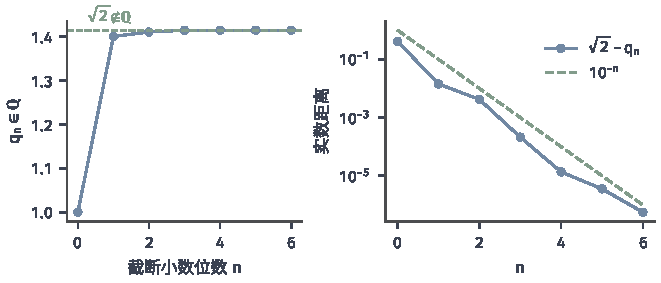
\includegraphics[width=112mm]{figures/01-mathematical-preliminaries-upper/01-mathematical-language-combinatorics-analysis-optimization/matplotlib/comprehension-additions/cauchy-completeness.pdf}
  \caption{由$\mathbb Q$在$\mathbb R$中稠密，对每个$n$选$a_n\in\mathbb Q$使$|a_n-\sqrt2|<1/n$。左图各项均为有理数，虚线是实数极限$\sqrt2$；右图的距离满足$0<\sqrt2-a_n<1/n$，用对数纵轴显示。有限个点不代替柯西性证明；该误差界与三角不等式才控制任意两个尾部项。}
  \label{fig:vol1-add-cauchy-completeness}
\end{figure}

再看$(0,1)$中的$1/n$（$n\geq2$）：它在环境实轴上趋于$0$，但$0$不在子空间中，
所以这列在$(0,1)$内缺少极限。两个例子共同说明，环境空间存在候选极限，并不保证子空间保有它。
稠密的$\mathbb Q$仍不完备，也区分了两件事：稠密描述对环境空间的任意精度逼近能力，完备描述对内部柯西列的极限保证。
接下来分别判断闭子集能否继承完备性，以及缺少极限的空间怎样扩充；
前面建立的双向距离界也可用来对应两侧柯西列，并据极限归属比较定义域与像的完备性。

\subsubsection{闭子集的完备性}
\label{sec:metric-closed-subspaces}

环境已经完备时，什么样的子集能够保留其中点列的极限？

\begin{theorem}[完备空间的闭子集完备]
\label{thm:metric-closed-subspace-complete}
设$X$完备，$A\subseteq X$为闭集，并配备子空间度量。则$A$完备。
\end{theorem}

\begin{proof}
任取$A$中的柯西列$(x_n)$。子空间度量与环境度量数值相同，所以它在$X$中仍是柯西列。
由$X$完备，存在$x\in X$使$x_n\to x$。再由闭集的序列判据~\eqref{eq:metric-sequential-closed}，$x\in A$。
于是该柯西列在$A$中收敛，$A$完备。
\end{proof}

环境完备负责“极限存在”，集合闭性负责“极限归属”，两步都不能省略。
空子集没有待检验的点列，按约定完备。
回看$(0,1)\subset\mathbb R$：环境完备，但子集没有保留趋于$0$的柯西列极限，这正是它不闭的后果。
若研究对象换成任意不完备空间，就不能只在原集合上宣布完备，而需要下一小节的扩张构造。

\subsubsection{度量空间的完备化}
\label{sec:metric-closed-subspaces-completion}

怎样用原空间的柯西列补入缺失的极限，并核对扩张后的空间确实完备？
先确定补入的点及点间距离，再把原空间安置进新空间，最后检验扩张空间能否保有任意柯西列的极限。

\paragraph{候选空间与度量}

先在度量空间$X$中收集全部柯西列，用它们表示可能缺失的极限候选。在柯西列之间定义
\[
  (x_n)\sim(y_n)\quad\Longleftrightarrow\quad d(x_n,y_n)\to0.
\]
自反性与对称性直接可得；若$(x_n)\sim(y_n)$、$(y_n)\sim(z_n)$，则
\[
  d(x_n,z_n)\leq d(x_n,y_n)+d(y_n,z_n)\to0,
\]
故传递性成立。以这些等价类组成候选空间
\[
  \widehat X=\bigl\{[(x_n)]:(x_n)\text{ 是 }X\text{ 中的柯西列}\bigr\}.
\]

接下来要为两个候选点规定距离。先固定两条柯西列$(x_n)$、$(y_n)$。反向三角不等式~\eqref{eq:metric-reverse-triangle}给出
\[
  \bigl|d(x_n,y_n)-d(x_m,y_m)\bigr|
  \leq d(x_n,x_m)+d(y_n,y_m).
\]
当$m,n$共同进入尾部时，右端任意小，所以实数列$\bigl(d(x_n,y_n)\bigr)$是柯西列；
由实数完备性，它有有限非负极限。于是可以定义
\begin{equation}
\label{eq:metric-completion-distance}
  D\bigl([(x_n)],[(y_n)]\bigr)=\lim_{n\to\infty}d(x_n,y_n).
\end{equation}

还要确认这个定义不依赖代表元。若$(x_n)\sim(u_n)$、$(y_n)\sim(v_n)$，则
\[
  \bigl|d(x_n,y_n)-d(u_n,v_n)\bigr|
  \leq d(x_n,u_n)+d(y_n,v_n)\to0,
\]
两个极限相等。对称性和三角不等式分别由原距离的相应性质取极限得到；而
\[
  D\bigl([(x_n)],[(y_n)]\bigr)=0
  \ \Longleftrightarrow\ d(x_n,y_n)\to0
  \ \Longleftrightarrow\ [(x_n)]=[(y_n)],
\]
分离性在类上恢复。因此$D$是$\widehat X$上的真正度量。

\paragraph{等距稠密嵌入}

把原空间的点映到常值列的等价类：令
\begin{equation}
\label{eq:metric-completion-embedding}
  i(x)=[(x,x,\ldots)].
\end{equation}
由式~\eqref{eq:metric-completion-distance}，
\[
  D(i(x),i(y))=\lim_{n\to\infty}d(x,y)=d(x,y),
\]
所以$i$保持距离，是\term{等距嵌入}（isometric embedding）；距离保持加上分离性使$i$单射。
后面始终保留映射$i$，不把原空间点与它的等价类暗中认成同一个对象。

原空间的像$i(X)$在$\widehat X$中稠密。固定新点$z=[(x_n)]$和$\varepsilon>0$。
因$(x_n)$是柯西列，存在$M$，使$m,n\geq M$时$d(x_m,x_n)<\varepsilon/2$。
固定任意$N\geq M$，对代表列的指标$n$取极限，得到
\[
  D(i(x_N),z)=\lim_{n\to\infty}d(x_N,x_n)\leq\frac{\varepsilon}{2}<\varepsilon.
\]
随着$N$增大，$i(x_N)$任意接近$z$，所以每个新点都在$i(X)$的闭包中。
这里“固定$N$、令$n$取极限”与“再让$N$增大”是两步不同操作，不能合并成一次取极限。

\paragraph{扩张空间的完备性}

\begin{theorem}[完备化]
\label{thm:metric-completion}
$\widehat X$是完备度量空间，且$i(X)$在$\widehat X$中稠密。
\end{theorem}

\begin{proof}
稠密性已经证明，只需证明$\widehat X$完备。任取$\widehat X$中的柯西列$(z_k)$。
由$i(X)$稠密，对每个$k$选原空间点$a_k\in X$，使
\[
  D(i(a_k),z_k)<2^{-k}.
\]
对任意$k,\ell$，等距性和三角不等式给出
\[
  d(a_k,a_\ell)=D(i(a_k),i(a_\ell))
  \leq 2^{-k}+D(z_k,z_\ell)+2^{-\ell}.
\]
当$k,\ell$共同进入尾部时，右端任意小，所以$(a_k)$是$X$中的柯西列。
这一步没有预先假定$z_k$已有极限。

令$z=[(a_k)]$，它是由上一柯西列给出的合法新点。把“等距稠密嵌入”中的常值类逼近用于代表列$(a_k)$，
有$D(i(a_k),z)\to0$。于是
\[
  D(z_k,z)\leq D(z_k,i(a_k))+D(i(a_k),z)<2^{-k}+D(i(a_k),z)\to0,
\]
即$z_k\to z$。每个$\widehat X$中的柯西列都有$\widehat X$内的极限，故$\widehat X$完备。
\end{proof}

构造至此给出等距稠密嵌入与\term{完备化}（completion）这一完备扩张；这里不额外声称已证明完备化在等距意义下唯一。

\subsubsection{双Lipschitz映射下的柯西列与完备性}
\label{sec:metric-map-cauchy-preservation}

双向距离界怎样对应两侧的柯西列，又怎样传递整个空间的完备性？
先对应两侧的列，再分别检查两个方向的极限落点。

\paragraph{柯西列的双向对应}

固定$f:D\subseteq X\to Y$满足式~\eqref{eq:metric-bilipschitz}。
上界使$D$中的柯西列映为像中的柯西列：若$(x_n)$柯西，则
\[
  d_Y(f(x_m),f(x_n))\leq C\,d_X(x_m,x_n)\to0.
\]
反过来，若像中的点列$y_n=f(x_n)$是柯西列，下界给出
\[
  d_X(x_m,x_n)\leq\frac1c\,d_Y(y_m,y_n)\to0,
\]
所以唯一的原像列也是柯西列；单射性保证“唯一原像”成立。

\paragraph{定义域与像的完备性}

在上述对应下，$D$与$f(D)$的完备性等价（像始终配备子空间度量）。

先设$D$完备。任取$f(D)$中的柯西列$y_n=f(x_n)$，由双向对应它的原像列$(x_n)$在$D$中柯西，
故$x_n\to x\in D$。再用上界，
\[
  d_Y(y_n,f(x))\leq C\,d_X(x_n,x)\to0,
\]
所以$y_n\to f(x)\in f(D)$，$f(D)$完备。这里是先拉回取极限，再用上界映出。

再设$f(D)$完备。任取$D$中的柯西列$(x_n)$，上界使$f(x_n)$成为像中的柯西列，
故它趋于某个$y\in f(D)$，可写$y=f(x)$且$x\in D$。下界给出
\[
  d_X(x_n,x)\leq\frac1c\,d_Y(f(x_n),f(x))\to0,
\]
所以$x_n\to x\in D$，$D$完备。
两个方向合起来得到$D$与$f(D)$完备性等价。
回看等距包含映射$j:(0,1)\to\mathbb R$：像$(0,1)$不完备而陪域$\mathbb R$完备，
因此只有满到整个陪域时，才能把像空间的结论表述为整个$Y$的结论。

\subsection{收敛子列与紧致性的序列刻画}
\label{sec:metric-compactness-tests}

现在任取点列，研究何时至少能得到一条在当前空间内收敛的子列。
本节回用集合节已经定义的紧致与全有界条件，证明紧致的序列刻画、
完备且全有界的联合判据，以及欧氏闭有界特例；这些等价证明把覆盖要求与极限保证连接起来。

\subsubsection{紧致与序列紧致}
\label{sec:metric-compact-sequential-tests}

此前的有限子覆盖条件，怎样等价于任意点列都能取到收敛子列？

若$K$中的每个点列都有一条收敛到$K$中某点的子列，就称$K$具有\term{序列紧致性}（sequential compactness）。
下面证明在度量空间中，紧致与序列紧致等价。
这是度量空间中的等价定理，不把结论外推到没有距离结构的任意拓扑空间。

\paragraph{紧致推出序列紧致}

先设$K$紧致，而$(x_n)$是$K$中的点列。
若不存在这样一个点，使它的每个邻域都含无穷多个序列指标，
则对每个$x\in K$都能取一个只含有限个指标的邻域$N_x$；
在其中选以$x$为中心的开球$U_x\subseteq N_x$，则$U_x$也只含有限个指标。
球族$\{U_x:x\in K\}$覆盖$K$，紧致性给出有限子覆盖$U_{x_1},\ldots,U_{x_N}$。
有限个“只含有限指标”的集合之并仍只含有限指标，与点列有无穷多个指标矛盾。

因此存在$x\in K$，使$x$的每个邻域都含无穷多个序列指标。
在$B(x,1/k)$中依次选取$n_k>n_{k-1}$，使$x_{n_k}\in B(x,1/k)$，便有$d(x_{n_k},x)<1/k$，
所以$x_{n_k}\to x$。这里计数的是序列指标；即使同一个取值重复出现，也能提供不同的指标。

\paragraph{序列紧致推出紧致}

再设$K$序列紧致，分两步推出开覆盖意义下的紧致。

第一步，序列紧致推出全有界。若某个$\varepsilon>0$没有有限个半径$\varepsilon$球覆盖$K$，
就可以递归选点：先选$x_1$，再从先前各点的$\varepsilon$球之外选$x_2$，如此继续，
使所得点列两两距离至少为$\varepsilon$。它的任何子列都不是柯西列，因而不可能收敛，与序列紧致矛盾。

第二步，证明对任意开覆盖$\mathcal U$，存在统一半径$r>0$，使每个$B(x,r)$都包含在某个覆盖成员中。
若不存在，对每个$n$选中心$x_n$，使$B(x_n,1/n)$不包含于任何$U\in\mathcal U$。
取收敛子列$x_{n_k}\to x$，并选$U_0\in\mathcal U$包含$x$；由$U_0$开，存在$R>0$使$B(x,R)\subseteq U_0$。
充分大的$k$同时满足$d(x_{n_k},x)<R/2$与$1/n_k<R/2$，三角不等式给出
\[
  B\!\left(x_{n_k},\frac1{n_k}\right)\subseteq B(x,R)\subseteq U_0,
\]
与$x_{n_k}$的选取方式矛盾，故统一半径$r$存在。

最后由全有界选有限个半径$r/2$的球覆盖$K$，设中心为$x_1,\ldots,x_N$。
每个$B(x_i,r)$都包含在某个原覆盖成员$U_i\in\mathcal U$中，
而$B(x_i,r/2)\subseteq B(x_i,r)\subseteq U_i$，所以$U_1,\ldots,U_N$覆盖$K$。
空空间的两种条件都直接成立。至此紧致与序列紧致等价。

\subsubsection{完备与全有界判据}
\label{sec:metric-complete-totally-bounded}

哪些空间条件能同时保证小尺度下不无限分散，并保住所构造子列的极限？

对空间$K$及其自身度量陈述结论：
\begin{theorem}[紧致的完备且全有界判据]
\label{thm:metric-complete-totally-bounded}
度量空间$K$紧致，当且仅当$K$完备且全有界。
\end{theorem}
若$K$是环境空间的子集，所有条件都按它的子空间度量解释，不能把环境的完备性直接移给$K$。

\paragraph{紧致空间的完备性}

集合节已经证明紧致推出全有界，只需再证紧致推出完备。
任取柯西列$(x_n)$。由紧致推出序列紧致，存在子列$(x_{n_k})$趋于某个$x\in K$。
给定$\varepsilon>0$，取$N$使$m,n\geq N$时$d(x_m,x_n)<\varepsilon/2$；
再取足够大的$k$，使$n_k\geq N$且$d(x_{n_k},x)<\varepsilon/2$。
于是对每个$n\geq N$，
\[
  d(x_n,x)\leq d(x_n,x_{n_k})+d(x_{n_k},x)<\varepsilon,
\]
所以整列收敛于$K$中的$x$，$K$完备。

\paragraph{完备且全有界空间的紧致性}

设$K$完备且全有界。对任意点列，逐层使用有限球覆盖：
第$j$层用有限个半径$2^{-j}$的球覆盖$K$，从上一层保留的无穷指标集中，
选出落入某个球的无穷子集。各层指标集逐层包含，但所选的球本身不必嵌套。

从第$j$层的指标集中选递增指标$n_j$，使$n_j$属于第$j$层选出的集合。
当$k,\ell\geq j$时，$x_{n_k}$与$x_{n_\ell}$都在第$j$层同一个半径$2^{-j}$的球中，
所以$d(x_{n_k},x_{n_\ell})<2^{1-j}$，子列$(x_{n_j})$是柯西列。
由完备性，它趋于某个$x\in K$；再由序列紧致与紧致的等价性，$K$紧致。

两个条件各负责一个不可省略的保证：$\mathbb R$完备却不全有界，$(0,1)$全有界却不完备。
可分性也不能代替全有界：可数无限离散空间可分（它本身可数）又有界，却不全有界，更不紧致。
另一方面，紧致空间由全有界及前面的有限网构造自动可分。因此有界与可分合起来，不能替代任意精度的有限覆盖。

\subsubsection{欧氏空间的闭有界判据}
\label{sec:metric-closed-bounded-limits}

利用点列与完备性，可以说明有限维欧氏空间的闭有界集为何紧致。
集合节已证明紧致在任意环境度量空间中都闭且有界，也给过无限离散空间的反例；
本小节只补欧氏空间的充分方向：对闭有界集分别取得完备性与全有界，再回用前一判据。

\paragraph{欧氏闭子集的完备性}

先证明$\mathbb R^d$完备。设$(\bm{x}_n)$是$\mathbb R^d$中的柯西列，记$\bm{x}_n=(x_{n,1},\ldots,x_{n,d})$。
由于
\[
  |x_{m,j}-x_{n,j}|\leq\lVert\bm{x}_m-\bm{x}_n\rVert_2,
\]
每个坐标列$(x_{n,j})_{n\geq1}$都是实数柯西列，由实数完备性有极限$x_j$。
令$\bm{x}=(x_1,\ldots,x_d)$。给定$\varepsilon>0$，让有限个坐标差同时小于$\varepsilon/\sqrt d$，则
\[
  \lVert\bm{x}_n-\bm{x}\rVert_2
  =\sqrt{\sum_{j=1}^{d}|x_{n,j}-x_j|^2}<\varepsilon,
\]
所以$\bm{x}_n\to\bm{x}$，$\mathbb R^d$完备。
由定理~\ref{thm:metric-closed-subspace-complete}，$\mathbb R^d$的闭子集配备子空间度量后也完备。

\paragraph{欧氏有界集的有限网}

再证明$\mathbb R^d$中的有界集全有界。设有界集$A$包含在一个有限边长的包围盒中。
对每个$\varepsilon>0$，用边长小于$\varepsilon/\sqrt d$的有限网格分割包围盒；
在每个与$A$相交的格子中选一个$A$内的点作为中心。
同一格子中任意两点的各坐标差都小于$\varepsilon/\sqrt d$，故欧氏距离小于$\varepsilon$，
这些有限个选点给出中心位于$A$中的有限$\varepsilon$网。
有限维性质在这里保证有限个坐标、有限个格子足以控制全体方向；空集可直接处理。

\paragraph{闭有界与紧致的等价}

把两条论证合并：闭性使$A$作为子空间完备，有界性使它全有界，
再由定理~\ref{thm:metric-complete-totally-bounded}，闭且有界的欧氏子集紧致。
与一般必要性合起来，得到有限维欧氏空间中的闭有界判据（Heine--Borel定理）：
\begin{equation}
\label{eq:metric-heine-borel}
  A\subseteq\mathbb R^d\text{ 紧致}\quad\Longleftrightarrow\quad A\text{ 闭且有界}.
\end{equation}

最后划定适用范围。在任意度量空间中，紧致都保证闭且有界；反向需要额外结构，
不能从欧氏特例直接外推，无限离散空间正说明闭且有界仍可缺少有限网。
一般判据始终是空间自身完备且全有界。

\subsection{压缩迭代的收敛与误差}
\label{sec:metric-contractive-solvers}

给定自映射$T:X\to X$，寻找满足$Tx_*=x_*$的点$x_*\in X$，称这样的点为$T$的不动点。
从起点$x^{(0)}$按
\[
  x^{(n+1)}=Tx^{(n)}
\]
生成候选点列以后，要研究它能否趋向这一目标，以及怎样控制误差。
迭代等式给出生成规则，压缩不等式则是保证点列收敛的条件。
在非空完备空间、自映射和统一压缩常数的共同条件下，先证明精确执行的结论，
再说明近似执行会增加哪些误差项。

\subsubsection{精确压缩迭代}
\label{sec:metric-exact-contraction}

本小节对同一迭代分别给出定性的不动点存在唯一性和定量的停止误差界。
这里建立的空间条件与误差估计，也将用于函数空间中求函数解的迭代。

\paragraph{不动点的存在与唯一}

对于目标方程$Tx_*=x_*$，什么条件能保证迭代$x^{(n+1)}=Tx^{(n)}$趋向唯一解？

\begin{definition}[不动点与压缩映射]
\label{def:analysis-fixed-point}
设$T:X\to X$为映射。点$x_*\in X$若满足$T(x_*)=x_*$，就称为$T$的\term{不动点}（fixed point）。
若存在$q\in[0,1)$，使所有$x,y\in X$满足
\begin{equation}
\label{eq:analysis-contraction-definition}
  d(Tx,Ty)\leq q\,d(x,y),
\end{equation}
就称$T$为\term{压缩映射}（contraction mapping），$q$称为压缩常数。
\end{definition}

压缩条件要求同一个严格小于$1$的常数在整个$X$上成立，并且$T$确实把$X$映回自身。

\begin{theorem}[Banach压缩映射定理]
\label{thm:analysis-banach-fixed-point}
设$(X,d)$是非空完备度量空间，$T:X\to X$是压缩常数为$q<1$的压缩映射。
则$T$有唯一不动点$x_*\in X$，并且从任意$x^{(0)}\in X$出发，由$x^{(n+1)}=Tx^{(n)}$生成的点列都收敛到$x_*$。
\end{theorem}

\begin{proof}
$q=0$时$T$为常值映射，一步即到不动点。以下设$0<q<1$。反复使用压缩条件，相邻两项满足
\[
  d\bigl(x^{(n+1)},x^{(n)}\bigr)
  \leq q\,d\bigl(x^{(n)},x^{(n-1)}\bigr)
  \leq q^n d\bigl(x^{(1)},x^{(0)}\bigr).
\]
对$m>n$，先用三角不等式串接相邻差，再求有限几何和：
\begin{align*}
  d(x^{(m)},x^{(n)})
  &\leq\sum_{j=n}^{m-1}d\bigl(x^{(j+1)},x^{(j)}\bigr)\\
  &\leq d\bigl(x^{(1)},x^{(0)}\bigr)\sum_{j=n}^{m-1}q^j\\
  &=\frac{q^n(1-q^{m-n})}{1-q}d\bigl(x^{(1)},x^{(0)}\bigr)
  \leq\frac{q^n}{1-q}d\bigl(x^{(1)},x^{(0)}\bigr).
\end{align*}
最后一个上界对所有$m>n$同时成立，并随$n$趋于零，所以迭代列是柯西列。
由完备性，存在$x_*\in X$使$x^{(n)}\to x_*$。压缩不等式~\eqref{eq:analysis-contraction-definition}还说明$T$连续，
因此$Tx^{(n)}\to Tx_*$；另一方面$Tx^{(n)}=x^{(n+1)}\to x_*$，
由极限唯一性得到$Tx_*=x_*$。这里先靠完备性取得候选极限，再靠映射的连续性验证它满足目标方程。

若$y_*$也是不动点，则
\[
  d(x_*,y_*)=d(Tx_*,Ty_*)\leq q\,d(x_*,y_*).
\]
由于$q<1$，只有$d(x_*,y_*)=0$，即$x_*=y_*$，不动点唯一。
\end{proof}

非空保证可以选择起点，自映射保证迭代能一直继续，完备性和严格压缩分别负责取得极限与收敛到不动点。
缺少条件时不能据此保证结论：在$(0,1)$上$T(x)=x/2$是严格压缩，但唯一可能的不动点$0$不在空间内；
在$\mathbb R$上$T(x)=x+1$只有Lipschitz常数$1$，它没有不动点。
这两个反例不是说缺少条件时所有问题都失败，而是说上述保证不再适用。

\paragraph{先验与后验误差界}

尚未知道不动点位置时，怎样从起点或已算相邻项估计当前误差？
记$e_n=d(x^{(n)},x_*)$。在证明中的尾和估计令$m\to\infty$，利用$x^{(m)}\to x_*$，得到先验界
\begin{equation}
\label{eq:analysis-banach-apriori-error}
  e_n\leq\frac{q^n}{1-q}d\bigl(x^{(1)},x^{(0)}\bigr).
\end{equation}
它只需要初始差和已知常数$q$，下标$n$从$0$开始计数。

从第$n$步起重新计算尾和，则得到后验界
\begin{equation}
\label{eq:analysis-banach-aposteriori-error}
  e_n\leq\frac{1}{1-q}d\bigl(x^{(n+1)},x^{(n)}\bigr).
\end{equation}
若只使用刚完成的两项且$n\geq1$，先用
$d(x^{(n+1)},x^{(n)})\leq q\,d(x^{(n)},x^{(n-1)})$控制尚未计算的下一步差，再代入上式，可得
\[
  e_n\leq\frac{q}{1-q}d\bigl(x^{(n)},x^{(n-1)}\bigr).
\]
两个式子对应不同数据条件：前者已知下一项，后者只知道当前项与前一项。

因此可以按目标误差$\varepsilon$，用式~\eqref{eq:analysis-banach-apriori-error}预先选择迭代步数，
也可以在每一步用式~\eqref{eq:analysis-banach-aposteriori-error}判断是否停止。
相邻差小只有结合收缩常数才成为误差证据：当$q$接近$1$时，因子$1/(1-q)$会放大上界，
不能只报告相邻差已经很小。

例如$T(x)=x/2+1$、$x^{(0)}=0$时，压缩常数$q=1/2$，$x^{(1)}=1$，唯一不动点是$2$。
先验界给出$|x^{(n)}-2|\leq2^{1-n}$，要求误差不超过$10^{-3}$时取$n=11$已足够；
后验界在这里化为$|x^{(n)}-2|\leq|x^{(n)}-x^{(n-1)}|$，无需事先知道答案$2$就能停止。
图~\ref{fig:vol1-add-contraction-cobweb}把这一迭代画成蛛网折线。
\begin{figure}[!htbp]
  \centering
  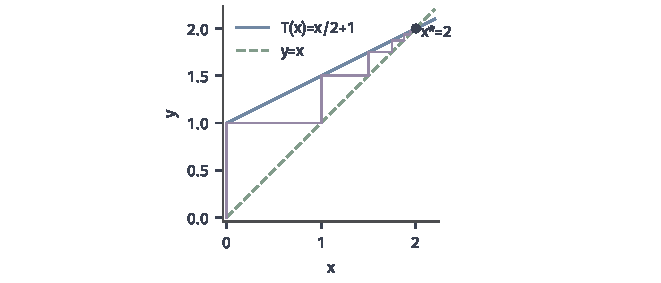
\includegraphics[width=112mm]{figures/01-mathematical-preliminaries-upper/01-mathematical-language-combinatorics-analysis-optimization/matplotlib/comprehension-additions/contraction-cobweb.pdf}
  \caption{$T(x)=x/2+1$在$[0,2]$上的七步迭代，初值$x^{(0)}=0$。蓝线是$T$，绿虚线是恒等函数，紫折线交替完成求值与复制；交点为$x_*=2$。精确迭代为$x^{(n)}=2-2^{1-n}$，图中的几何收缩对应压缩常数$1/2$。}
  \label{fig:vol1-add-contraction-cobweb}
\end{figure}

以上结论都假定精确执行$x^{(n+1)}=Tx^{(n)}$。若一次执行带有误差，
应把该误差单独写入递推再估计，不能直接照抄精确后验界；这就是下一小节的内容。

\subsubsection{带扰动的压缩迭代}
\label{sec:metric-perturbed-contraction}

每一步都只能近似执行压缩映射时，误差会消失还是累积到某个水平？
先跟踪每步执行误差的传播，再在不同扰动条件下估计极限行为，最后用已算数据认证当前精度。

\paragraph{扰动误差的递推与传播}

保持非空完备空间、自映射$T$与统一压缩常数$0\leq q<1$。
现在$x^{(n)}$表示近似执行得到的点列，每个计算点仍在$X$中，并满足
\begin{equation}
\label{eq:analysis-perturbed-execution}
  d\bigl(x^{(n+1)},Tx^{(n)}\bigr)\leq\eta^{(n)},\qquad \eta^{(n)}\geq0.
\end{equation}
以前项已证明存在唯一的精确不动点$x_*$为参照，令$e_n=d(x^{(n)},x_*)$。
由三角不等式和$Tx_*=x_*$，
\[
  e_{n+1}
  \leq d\bigl(x^{(n+1)},Tx^{(n)}\bigr)+d\bigl(Tx^{(n)},Tx_*\bigr)
  \leq \eta^{(n)}+q e_n,
\]
即
\begin{equation}
\label{eq:analysis-perturbed-distance-recursion}
  e_{n+1}\leq q e_n+\eta^{(n)}.
\end{equation}
% 保留内容迁移前的语义标签，指向同一公式。
\begingroup
\makeatletter
\let\label\ltx@label
\label{eq:prelim-perturbed-recurrence}
\endgroup
右边清楚区分了旧误差的收缩与本步新增误差。

先代入两步核对：
\[
  e_1\leq qe_0+\eta^{(0)},\qquad
  e_2\leq q^2e_0+q\eta^{(0)}+\eta^{(1)}.
\]
由同一递推归纳得到
\begin{equation}
\label{eq:analysis-perturbed-distance-unrolling}
  e_n\leq q^n e_0+\sum_{j=0}^{n-1}q^{\,n-1-j}\eta^{(j)}.
\end{equation}
% 保留内容迁移前的语义标签，指向同一公式。
\begingroup
\makeatletter
\let\label\ltx@label
\label{eq:prelim-unrolled-recurrence}
\endgroup
第$j$步加入的误差$\eta^{(j)}$经过此后$n-1-j$次收缩，因而带上相应幂次$q^{n-1-j}$。
前两步展开也可用来核对求和的起止下标与最新误差项的权重。

\paragraph{扰动误差的渐近估计}

若所有执行误差都有统一上界$\eta^{(j)}\leq\eta$，有限几何和给出
\[
  e_n\leq q^n e_0+\eta\frac{1-q^n}{1-q},
\qquad
  \limsup_{n\to\infty}e_n\leq\frac{\eta}{1-q}.
\]
这是误差的上界，不是实际误差的等式，也不是不可突破的下界；它不保证点列或误差列一定有极限。
当$q$接近$1$时，同样的执行误差对应更大的保证范围。

若$\eta^{(j)}\to0$，则$e_n\to0$。给定$\varepsilon>0$，先固定$J$，使$j\geq J$时
$\eta^{(j)}\leq(1-q)\varepsilon/2$。式~\eqref{eq:analysis-perturbed-distance-unrolling}的加权和中，
$j\geq J$的晚期部分由几何和控制在$\varepsilon/2$以内；$j<J$的早期部分只有有限项，
其权重随$n$衰减，连同$q^ne_0$在充分大的$n$时小于$\varepsilon/2$。
可求和误差是保证误差趋零的一项更强条件，它与“误差列趋零”并不互斥：趋零已经足够，可求和时估计通常更整齐。

\paragraph{带扰动的后验误差界}

还可以把已知执行误差转成可计算的停止界。由$Tx_*=x_*$与压缩条件，
\[
  e_n=d(x^{(n)},x_*)\leq d(x^{(n)},Tx^{(n)})+d(Tx^{(n)},Tx_*)\leq d(x^{(n)},Tx^{(n)})+q e_n,
\]
所以
\begin{equation}
\label{eq:metric-perturbed-residual-bound}
  e_n\leq\frac{1}{1-q}d(x^{(n)},Tx^{(n)}).
\end{equation}
若已算出$x^{(n+1)}$并有本步界$\eta^{(n)}$，则
$d(x^{(n)},Tx^{(n)})\leq d(x^{(n+1)},x^{(n)})+\eta^{(n)}$，代入得到
\begin{equation}
\label{eq:metric-perturbed-posterior-next}
  e_n\leq\frac{d(x^{(n+1)},x^{(n)})+\eta^{(n)}}{1-q},
\end{equation}
它认证的是点$x^{(n)}$。若要用刚完成的第$n-1$步直接认证$x^{(n)}$，则在$n\geq1$时把上一步界代入递推：
\[
  e_n\leq q\,e_{n-1}+\eta^{(n-1)}
  \leq\frac{q\,d(x^{(n)},x^{(n-1)})+\eta^{(n-1)}}{1-q}.
\]

\begin{example}[持续扰动与衰减扰动]
\label{ex:prelim-recurring-perturbations}
取$e_0=1$、$q=1/2$，并暂把递推中的不等号取为等号。若每步都加入$\eta^{(j)}=0.1$，则
\[
  e_n=2^{-n}+0.1\sum_{j=0}^{n-1}2^{-j}=0.2+0.8\cdot2^{-n},
\]
初始误差逐步消失，持续加入的误差却留下$0.2$的极限上界。若改为$\eta^{(j)}=0.1/(j+1)$，
扰动本身衰减，稳定递推使$e_n\to0$。例如第$1$步两者都是$0.6$，第$2$步分别为$0.4$和$0.35$；
差别来自第二步加入的新误差，而不是初值不同。
\end{example}
图~\ref{fig:prelim-perturbed-recurrence}比较了两种递推的轨迹。
\begin{figure}[htbp]
  \centering
  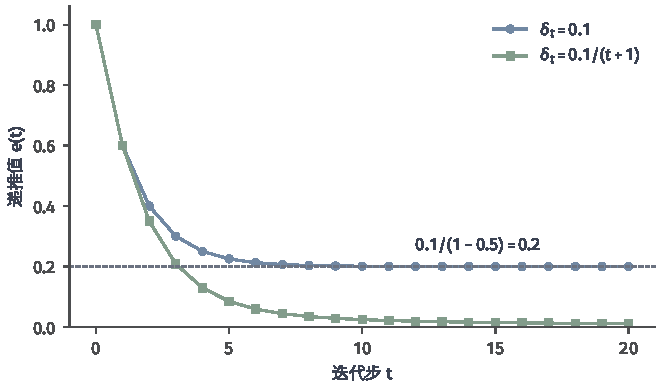
\includegraphics[width=112.0mm]{figures/01-mathematical-preliminaries-upper/01-mathematical-language-combinatorics-analysis-optimization/matplotlib/prelim-perturbed-recurrence/figure.pdf}
  \caption{相同初值与收缩系数下的两种递推。蓝线使用持续扰动，绿线使用衰减扰动；每个点都是整数步上的精确递推值，灰虚线是持续扰动留下的极限$0.2$。图为教学构造。}
 \label{fig:prelim-perturbed-recurrence}
\end{figure}

最后要核对停止结论依赖的资料：必须有同一个精确映射$T$、可用的统一常数$q$和相应执行误差界，
且近似点始终留在$X$中，才能把残差或相邻步长变成上述保证。
这里不把一般不稳定迭代或未知映射误差纳入已证明的压缩结论；
误差趋零的长期极限结论，与某一步达到指定精度的认证，也分别使用相应条件。

\section{本章小结}
\label{sec:metric-summary}

本章从度量规则进入集合、映射和点列。
集合侧用邻域与开闭集说明位置关系，用稠密子集说明任意精度的逼近，
再区分一套可数稠密代表与每个精度下的有限$\varepsilon$网。
全有界推出有界和可分，有界加可分仍不足以推出全有界；
紧致则以任意开覆盖都有有限子覆盖为正式定义，紧致集在环境空间中闭、有界、全有界且可分。

映射侧区分逐点连续、一致连续、Lipschitz与双Lipschitz所要求的距离控制。
连续映射把紧致定义域映成紧致像；定义域非空时，实值连续函数因而取得极值，
连续映射在紧集上还获得一致连续性。这些存在性与连续性结论本身不保证极值或最近点唯一，也不提供求解算法。
双Lipschitz的双侧界保持收敛与柯西性，并给出定义域和其像在各自子空间度量下的完备性等价；
等距包含映射提醒我们，没有满到整个陪域时不能把像的性质推广到陪域。

点列侧，收敛列必为柯西列，而在完备空间中每个柯西列都收敛。
完备空间的闭子空间继承完备性；完备化则把原空间等距而稠密地嵌入一个完备空间。
紧致空间保证任意点列存在收敛子列；在度量空间中，这一序列刻画等价于开覆盖定义，
也导出“完备且全有界”的一般判据。欧氏空间的闭有界判据依靠有限维空间提供有限网，
不能直接外推到一般度量空间。

最后，把自映射的反复执行看成生成点列的具体规则。
非空、完备、自映射和统一压缩常数共同保证唯一不动点，并给出精确迭代的先验与后验误差界；
带扰动执行还要追踪每步误差及其几何权重，统一误差留下$\eta/(1-q)$的保证范围，衰减误差则可使总误差趋零。
后章采用完备、可分等背景时，应核对实际选定的度量是否满足这些条件，
并保留它们与紧致性的区别，不能单凭可分性或有界性补足极限保证。

\FloatBarrier
